\documentclass[14pt, dvipsnames, twoside]{extarticle}
\usepackage[left=2cm, top=2.5cm, right=2cm, bottom=20mm]{geometry} 
\usepackage[utf8x]{inputenc} % Включаем поддержку UTF8
\usepackage[russian]{babel}  % Включаем пакет для поддержки русского языка
\usepackage{ucs}
\usepackage{tikzsymbols}
 \usepackage{fontawesome}
 \usepackage{simpsons}
 \usepackage{xcolor}
  \usepackage{stackrel}
 
\usepackage{wrapfig}
  
\usepackage{amsthm, amsmath, amssymb} % Mathematical typesetting

\usepackage{esint}
 
\newtheorem{theorem}{Теорема}
\newtheorem{statement}{Утверждение}
\newtheorem{proposition}{Предложение}
\newtheorem{lemma}{Лемма}
\newtheorem{corollary}{Следствие}[theorem]
\newtheorem{question}{Вопрос}


\theoremstyle{definition}
\newtheorem{defi}{Определение}
\newtheorem{property}{Свойство}
\newtheorem{problem}{Задача}
\newtheorem{exercise}{Упражнение}
\newtheorem{example}{Пример}

\theoremstyle{remark}
\newtheorem*{comment}{Замечание}
\newtheorem*{hypothesis}{\bf Гипотеза}
\newtheorem*{construction}{Конструкция}

\usepackage{enumerate}











\usepackage{asymptote}

\usepackage[all]{xy}

\DeclareMathOperator{\Tor}{\mathrm{Tor}\!}
\DeclareMathOperator{\End}{\mathrm{End}\,}
\DeclareMathOperator{\Sq}{\mathrm{Sq}}
\DeclareMathOperator{\cp}{\smallsmile}
\DeclareMathOperator{\Hom}{\mathrm{Hom}}
\DeclareMathOperator{\Sp}{\mathrm{Sp}}
\DeclareMathOperator{\Z2}{\mathbb{Z}_2}
\DeclareMathOperator{\Ho}{\mathrm{Ho}}
\DeclareMathOperator{\CC}{\mathbb{C}\!}
\DeclareMathOperator{\Hig}{\mathrm{Hig}}

\renewcommand{\phi}{\varphi}

\usepackage{textcomp}

\usepackage{mathabx}

%Некий костыль с двух сторон от декларации пакета bm
\let\saveboldsymbol\boldsymbol
\usepackage{bm}
\let\boldsymbol\saveboldsymbol

\usepackage{mathrsfs} 

\usepackage{indentfirst}

  \usepackage{multicol}

\newcommand{\factor}[2]{{\raisebox{.2em}{$#1$}\left/\raisebox{-.2em}{$#2$}\right.}}

\usepackage{titlesec}
\titleformat{\section}
  {\normalfont\Large\bfseries}{\S\thesection}{1em}{}

  
  
  
\usepackage{hyperref} % For hyperlinks in the PDF 
\usepackage{fancybox,fancyhdr}
\usepackage{lipsum}
\pagestyle{fancy}


%\usepackage[nottoc,numbib]{tocbibind}






\usepackage{array}
\newcolumntype{P}[1]{>{\centering\arraybackslash}p{#1}}




\usepackage{caption}



\hypersetup{
  colorlinks   = true, %Colours links instead of ugly boxes
  urlcolor     = black, %Colour for external hyperlinks
  linkcolor    = black, %Colour of internal links
  citecolor   = black %Colour of citations
}





%\makeatletter
%\def\@cite#1#2{[\textbf{#1\if@tempswa , #2\fi}]}
%\def\@biblabel#1{[\textbf{#1}]}
%\makeatother











\begin{document}

\renewcommand{\sectionmark}[1]{ \markboth{#1}{}} 

\captionsetup[figure]{labelfont={it},labelformat={default},labelsep=period,name={Рис.}}









\thispagestyle{empty}
\begin{center}
\sc Федеральное государственное бюджетное образовательное \\
учреждение высшего образования \\
<<Московский государственный университет \\
\textnormal{имени} М. В. Ломоносова>>
\end{center}

\begin{center}
\sc механико-математический факультет
\end{center}

\begin{center}
\sc кафедра высшей геометрии и топологии
\end{center}





\hfill\break





\begin{center}
\sc выпускная квалификационная работа \\
(дипломная работа) \\
\textnormal{специалиста}
\end{center}

\begin{center}
\textsc{\textbf{Торическая топология \\ ациклических симплициальных комплексов}}
\end{center}

\hfill\break


\begin{flushright}
Выполнил студент \\
605 группы \\
Корнев Михаил Игоревич \\
\hfill\break

\begin{tabular}{@{}P{.1in}P{3in}@{}}
& \hrulefill \\
& подпись студента
\end{tabular}

\end{flushright}






\begin{flushright}
Научный руководитель: \\
чл.-кор. РАН, профессор  \\
Бухштабер Виктор Матвеевич \\
\hfill\break

\begin{tabular}{@{}P{.1in}P{3in}@{}}
& \hrulefill \\
& {\centering подпись научного руководителя}
\end{tabular}

\end{flushright}




\vspace*{\fill}

\begin{center}
Москва \\
2022
\end{center}


 
\clearpage
~
\thispagestyle{empty}
\clearpage
     
\newpage





















\thispagestyle{empty}



\tableofcontents

\thispagestyle{empty}

\newpage

















\fancyhf{}
%\fancyhead[LE,RO]{\thepage}
%\fancyhead[RE,LO]{\S\thesection. \leftmark}
%\fancyfoot[CE,CO]{}
%\fancyfoot[LE,RO]{}

\rhead{\thepage}
\lhead{\S\thesection. \leftmark}



\section{Введение}\label{Introduction}

\subsection{Актуальность исследования}


В химии фуллереном называется молекула, которая представляет собой выпуклый многогранник с атомами углерода в вершинах, принадлежащих в точности трём углеродным кольцам длины 5 или 6. Математически фуллерен является трёхмерным выпуклым многогранником, все грани которого пяти- и шестиугольники, а в каждой вершине сходится ровно по три ребра (последнее условие является определением простого многогранника) \cite{Fullerenes}. 

Проблема классификации изомеров фуллеренов очень важна применительно к химии, физике, биологии и нанотехнологиям. В этой связи последнее время активно развивается математическая теория фуллеренов \cite{Bille, StructuralChemistry}. Два изомера фуллерена считаются неотличимыми, если соответствующие многогранники имеют изоморфные решётки граней.

Простой трёхмерный многогранник называется погореловским, если он допускает реализацию в виде ограниченного многогранника с прямыми двугранными углами в трёхмерном пространстве Лобачевского \cite{ErokhovetsFullerenes}. В торической топологии имеется результат \cite{Fullerenes} о том, что два погореловских многогранника комбинаторно эквивалентны тогда и только тогда, когда изоморфны кольца когомологий соответствующих данным многогранникам момент-угол многообразий. Известно \cite{Fullerenes}, что фуллерены являются погореловскими многогранниками, поэтому для них также справедлив данный результат. Таким образом, с каждым фуллереном можно ассоциировать алгебраическую структуру, которая однозначно характеризует его решётку граней. 

Сопоставление фуллерену некоторого кольца мотивирует следующую конструкцию. Для каждого выбора семейства ацикличных групп $\{A_i\}$ имеется функтор $T$, впервые введённый Дэниелем Каном и Уильямом Тёрстоном в \cite{Kan}, 1976 (см. также \cite{BDH, Maunder}). Функтор $T$ сопоставляет полиэдральному разбиению $P$ пространства $X$ асферическое пространство $TX = K(G_P, 1)$ с такими же гомологиями и когомологиями, как у пространства $X$. Значит, каждому конечному полиэдральному разбиению пространства $X$ функториально соответствует конечно определённая группа $G_P$.

В контексте конструкции функтора Кана-Тёрстона представляют интерес ацикличные группы. По определению это группы, гомологии которых устроены так же, как гомологии точки. В работах \cite{View, BerrickHillman, BDH, BaumslagUniversal} представлены известные результаты о таких группах и их роль в алгебраической топологии и комбинаторной теории групп. В частности, в работе трёх авторов \cite{BaumslagUniversal}, 1983 представлена конструкция универсальной конечно определённой ацикличной группы, использующая, в свою очередь, конструкцию универсальной  группы из работы Хигмана \cite{UniversalHigmanGroup}, 1961. Последняя группа не имеет явного описания, и работа \cite{ExplicityPresentation}, 2016 устраняет этот недостаток, предъявляя более явное задание с 8-ю образующими и 26-ю соотношениями. Наиболее известной ацикличной группой является группа $\Hig_4$, построенная вместе с группами $\Hig_n$, $n\geqslant 5$ в работе Хигмана \cite{Higman}, 1951. Однако там группы $\Hig_n$ рассматриваются, как примеры конечно определённых групп, не содержащих нетривиальных собственных нормальных подгрупп конечного индекса, и факт об ацикличности $\Hig_n$ не приводится. Первое упоминание об ацикличности группы $\Hig_4$, по-видимому, встречается в работе \cite{BDH}, 1980.   










\subsection{Цель и задачи исследования}



 

{\bf Цель научного исследования:} исследование свойств ацикличных групп и соответствия $P\mapsto G_P$ для  полиэдральных разбиений $P$ пространства $X$.

{\bf Задачи научного исследования:}

\begin{enumerate}[\bf 1.]

\item Исследовать свойства ацикличных конечно определённых групп.

\item Описать копредставление соответствующей группы $G_P$ по данному полиэдральному разбиению $P$ клеточного пространства $X$. 

\item Исследовать соответствие $P\mapsto G_P$ в контексте изомеров фуллеренов.

\iffalse
\item Применить соответствие $P\mapsto G(P)$ к описанию классификации фуллеренов, где $P$ является границей фуллерена.
\fi  

\end{enumerate}











\subsection{Методы исследования}

В ходе исследования использованы и развиты методы комбинаторной теории групп и алгебраической топологии.












\subsection{Результаты исследования}


\begin{enumerate}[\bf 1.]

\item Построено бесконечное семейство примеров неасферичных ацикличных пространств. Замечено, что универсальной ацикличной группой может служить группа, имеющая задание с 12 образующими и 38 соотношениями.  Для произвольной дискретной группы $G$ построено нестягиваемое ацикличное пространство $\mathcal{E}G$, на котором группа $G$ действует свободно.

\item Дан алгоритм построения конечно определённой группы $G_P$ для любого конечного полиэдрального разбиения $P$ клеточного пространства $X$.

\item Дан алгоритм построения по каждому фуллерену $P$ с фиксированной ориентацией и данному ориентированному гамильтонову пути конечно определённой группы $G_P$. 

\end{enumerate}
















\section{Напоминание о гомологиях дискретных групп}

В настоящей работе, если не оговорено противное, все встречающиеся группы предполагаются дискретными, то есть рассматриваются в дискретной топологии.

По группе $G$ можно, как известно, построить стягиваемый симплициальный комплекс $EG$ со свободным действием $G$. Факторпространство $BG:=\factor{EG}{G}$ называется {\it классифицирующим пространством} группы $G$. Существуют различные конструкции классифицирующих пространств для топологических и дискретных групп. Сюда относится конструкция с джойнами Милнора \cite{MilnorBG}, конструкция Милграма \cite{Milgram}, категорная конструкция через геометрическую реализацию некоторого симплициального множества \cite{Jardine} и др. 

Классифицирующее пространство дискретной группы $G$ имеет тип пространства Эйленберга-Маклейна $K(G, 1)$ \cite{Hatcher}. Напомним, что пространство $K(G, 1)$ с точностью до гомотопической эквивалентности определяется из условий:\\ $\pi_n(K(G, 1)) = 0$, если $n > 1$ и $\pi_1(K(G, 1)) = G$. 

\begin{defi}\label{group_homology_BG}
{\it Гомологиями дискретной группы $G$ с тривиальными коэффициентами $\mathbb{Z}$} называются гомологии (симплициальные, клеточные и др.) классифицирующего пространства группы $G$, то есть $H_i(G; \mathbb{Z}):=H_i(BG; \mathbb{Z})$. В случае локальных коэффициентов в $G$-модуле $M$, это гомологии с локальными коэффициентами $H_i(BG; M)$.
\end{defi}

Также гомологии группы $G$ могут быть определены чисто алгебраическим путём:

\begin{defi}\label{group_homology_resolution}
{\it Гомологиями дискретной группы с коэффициентами в $G$-модуле $M$} называются группы $H_n(G, M)=\mathrm{Tor}^{\mathbb{Z}[G]}_n(\mathbb{Z}, M)$.
\end{defi}


\begin{statement}[см., например, \cite{Brown}]
Два определения \ref{group_homology_BG} и \ref{group_homology_resolution} гомологий групп равносильны.
\end{statement}

%С каждым гомоморфизмом групп $G_1\to G_2$ связано расслоение $\factor{G_2}{G_1}\to BG_1\to BG_2$.

 Имеется следующий класс групп, не только важный для дальнейшего, но представляющий и самостоятельный интерес:
 
 
\begin{defi}
Группа $G$ называется {\it ацикличной}, если её гомологии в тривиальном $G$-модуле $\mathbb{Z}$ устроены, как гомологии точки, т. е. $$H_\ast(G) \cong H_\ast(\mathrm{pt}).$$
\end{defi}
 
 
 Заметим, что ацикличных групп относительно любой локальной системы коэффициентов не существует. Действительно, иначе по лемме Шапиро \cite{Brown} мы бы имели изоморфизм $$H_1(G, \mathbb{Z}[G/C]) \cong H_1(C) \cong C $$ для нетривиальной циклической подгруппы $C < G$. 
 
 В силу этого наблюдения, если не оговорено противное, под ацикличностью группы $G$ будет пониматься именно ацикличность $G$ относительно тривиального $G$-модуля $\mathbb{Z}$.
 




























\section{Примеры ацикличных дискретных групп}

Ацикличные группы могут возникать, как группы автоморфизмов больших объектов. Так, ацикличными является группа гомеоморфизмов $\mathbb{R}^n$ с компактными носителями \cite{Mather} (в дискретной топологии), группа $\mathrm{GL}(V)$ обратимых преобразований бесконечномерного гильбертова пространства \cite{Automorphisms} (в дискретной топологии).

В маломерной топологии ацикличные группы могут встречаться, например, в качестве коммутантов групп узлов с тривиальными полиномами Александера \cite{View} или как некоторое расширение группы кос на бесконечном числе нитей \cite{BerrickHillman}.

В этом параграфе приводятся явные конструкции из \cite{BDH} конечно представленных ацикличных групп, классифицирующие пространства которых могут быть реализованы двумерными симплициальными комплексами. 

\subsection{Группа $\mathfrak{A}$} 


Рассмотрим простой пример нетривиальной ацикличной группы --- группу $\mathfrak{A}$.

Для её построения сначала введём две группы: $$F=\langle a, b \rangle,$$ $$C=\langle u=a,\ v=b^{-1}a^{-1}bab,\ w=b^{-2}ab^{-1}a^{-2}bab^2,\ x= b^{-3}ab^{-1}a^{-2}bab^3 \rangle.$$

Группа $F$ --- свободная на двух образующих, а группа $C$ --- свободная на четырёх образующих.

При помощи $F$ и $C$ мы можем получить группу $$\mathfrak{A}=\{ F_1\star F_2; C_1\cong_\varphi C_2\},$$ где $F_1, \ F_2$ --- две копии группы $F$, а $C_1$, $C_2$ --- копии группы $C$, причём склейка происходит вдоль изоморфизма $\varphi: C_1\to C_2$, такого, что $$u_1\mapsto x_2,\ v_1\mapsto w_2,\ w_1\mapsto v_2,\ x_1\mapsto u_2.$$ 

\begin{statement}
Группа $\mathfrak{A}$ нетривиальна.
\end{statement} 

\begin{proof}
Свободные группы нетривиальны, поскольку имеют нетривиальные первые гомологии (совпадающие с гомологиями букета окружностей). Но результат амальгамированного произведения двух нетривиальных групп по их общей подгруппе будет нетривиальной группой. Последнее следует из теоремы о нормальной форме для свободных произведений групп над общей подгруппой (см., например, \cite{Serre}).
\end{proof}

\begin{statement}[\cite{BDH}] 
Группа $\mathfrak{A}$ является ацикличной.
\end{statement}

\begin{proof}

По построению группа $\mathfrak{A}$ является совершенной.

Кроме того, пространство $K(\mathfrak{A}, 1)$ можно реализовать в виде конечного клеточного двумерного комплекса, поскольку оно является пушаутом двух копий пространства $K(F, 1)\simeq \mathbb{S}^1\vee \mathbb{S}^1$ вдоль пространства $K(C, 1)\simeq \mathbb{S}^1\vee\mathbb{S}^1\vee\mathbb{S}^1\vee\mathbb{S}^1$, то есть $$K(\mathfrak{A}, 1)=K(F, 1)\sqcup_{K(C, 1)} K(F, 1).$$ 

Имеет место точная последовательность Майера-Виеториса с постоянными коэффициентами $\mathbb{Z}$ 
$$...\to H_{n+1}\mathfrak{A}\to H_nC\to H_nF_1\oplus H_n F_2\to H_n\mathfrak{A}\to ...$$

В силу того, что $K(F, 1)$ и $K(C, 1)$ --- букеты окружностей, сразу получается, что $H_n\mathfrak{A}=0$ при $n>2$. Рассмотрим теперь участок точной последовательности для случая $n=2$: 
$$0\to H_2\mathfrak{A}\to H_1C\to H_1F_1\oplus H_1F_2\to 0.$$ Но обе свободные абелевы группы $H_1C$ и $H_1F_1\oplus H_1 F_2$ имеют ранг 4. Следовательно, эпиморфизм между ними является изоморфизмом, и $H_2\mathfrak{A}=0$ в силу точности.


\end{proof}

Для дальнейшего нам понадобится важная

\begin{theorem}[Дж. Уайтхед, 1939, \cite{Whitehead}]\label{Whitehead}
Пусть группа $G$ является копределом в категории $\mathbf{Group}$ следующей диаграммы 

$$\xymatrix{
    C \ar@{^{(}->}[r] \ar@{^{(}->}[d] & A \ar@{-->}[d] \\
    B \ar@{-->}[r]       & G }$$ 
    
Тогда пространство $K(G, 1)$ является копределом в категории $\mathbf{Top}$ диаграммы  

$$\xymatrix{
    K(C, 1) \ar[r] \ar[d] & K(A, 1) \ar@{-->}[d] \\
    K(B, 1) \ar@{-->}[r]       & K(G, 1) }$$ 
    
\end{theorem}

\begin{corollary}[\cite{BDH}]\label{finite}
Пусть $G=A\star_C B$ является свободным произведением групп $A$ и $B$ с объединённой подгруппой $G$. Предположим, что для групп $A$, $B$, $C$ существуют конечные симплициальные комплексы $K(A, 1)$, $K(B, 1)$ и $K(C, 1)$. Тогда $K(G, 1)$ тоже может быть реализовано в виде конечного симплициального комплекса. Причём имеет место оценка на размерности $$\dim G\leqslant \max(\dim A, \dim B, 1+\dim C).$$
\end{corollary} 

\begin{proof}

Вложениям $C\hookrightarrow A$ и $C\hookrightarrow B$ соответствуют отображения классифицирующих пространств $K(C, 1)\to K(A, 1)$ и $K(C, 1)\to K(B, 1)$. Возьмём цилиндры этих отображений и склеим их вдоль комплекса $K(C, 1)$.
\end{proof}

Отсюда получается  

\begin{statement}[\cite{BDH}]
Группа $\mathfrak{A}$ является ацикличной относительно тривиальной системы коэффициентов в $\mathbb{Z}$ и может быть реализована в виде конечного двумерного клеточного комплекса.
\end{statement}











\subsection{Группы Хигмана $\boldsymbol{\mathrm{Hig}_n}$}

Эти группы были предложены Г. Хигманом в работе \cite{Higman}, 1951, как примеры конечно определённых групп, не имеющих нетривиальных собственных подгрупп конечного индекса.

\paragraph{Случай $\bm{n = 4}$.} Рассмотрим группу

$$\mathrm{Hig}_4=\langle a, b, c, d\ |\ a^{-1}ba=b^2, b^{-1}cb=c^2, c^{-1}dc=d^2, d^{-1}ad=a^2 \rangle.$$ 

Опишем, как можно получить эту группу при помощи операций HNN-расширения и амальгамированного свободного произведения.

Рассмотрим группу Баумслага-Солитера: $$K := \mathrm{BS}(1,2)=\langle a, b\ |\ a^{-1}ba=b^2 \rangle.$$

Группа $K$ является HNN-расширением группы $\langle b \rangle\cong\mathbb{Z}$ при помощи изоморфизма подгрупп $\langle b \rangle \cong \langle b^2 \rangle$. Заметим, что из теоремы о нормальной форме для HNN-расширений \cite{Serre} следует, что группа $K$ ненулевая, поскольку в неё вкладывается группа $\langle a \rangle$. 

%Также из леммы Бриттона следует, что если бы $K$ имела элемент кручения, то он был бы сопряжён некоторому элементу группы $\mathbb{Z}$, значит, $K$ не имеет кручения.  

Дайер и Васкез показали, что верна

\begin{theorem}[E. Dyer, A. T. Vasquez, 1972, \cite{Vasquez}]\label{Vasquez}

Пусть $P=\langle S\ |\ r \rangle$ --- представление группы $G$ с одним соотношением $r\in F(S)$, и $r$ не является степенью (большей 1) никакого слова. Тогда клеточный двумерный комплекс, получаемый стандартной приклейкой двумерной клетки к букету окружностей, биективно соответствующих образующим из $S$ вдоль слова $r$, асферичен.

\end{theorem}



\begin{corollary}[\cite{BDH}]
Классифицирующим пространством группы $K$ является двумерный комплекс, получаемый из букета двух окружностей некоторой приклейкой двумерной клетки. 
\end{corollary}

Из теорем Хопфа (см. например, \cite{Brown}) очевидно следует, что $H_2(K)=0$ и $H_1(K)=\mathbb{Z}$. Следовательно, мы знаем гомологии группы $K$:

\begin{proposition}
$$\begin{cases}
H_{n}(K)=0, & n\geqslant2,\\
H_{1}(K)=\mathbb{Z}
\end{cases}$$
\end{proposition}

Построим группу $$L= K_1\star_{\mathbb{Z}} K_2=\langle a, b, c\ |\  a^b=a^2, b^c=b^2 \rangle,$$ где $K_i\cong K$, и склейка происходит вдоль вложений $\mathbb{Z}\cong \langle a \rangle\hookrightarrow L$ , $\mathbb{Z}\cong\langle b \rangle\hookrightarrow L$. Очевидно, что $H_1(L)=\mathbb{Z}$. Из точной последовательности Майера-Виеториеса и предложения выше следует, что $H_n(L)=0$ при $n\geqslant 2$.

Возьмём амальгаму $L_1\star_{\mathbb{Z}\star\mathbb{Z}} L_2$, где $L_i\cong L$, со склейкой $\langle a_1, c_1 \rangle \cong \langle a_2, c_2 \rangle$ и получим группу Хигмана $\mathrm{Hig}_4$.

Из теоремы Уайтхеда \ref{Whitehead} и теоремы Дайера-Васкеза \ref{Vasquez} следует, что $K(\Hig_4, 1)$ представляет собой двумерный клеточный комплекс с одной нульмерной клеткой, четырьмя одномерными клетками и четырьмя двумерными клетками.


Приведём здесь явную конструкцию симплициального комплекса, являющегося классифицирующим пространством группы Хигмана $\Hig_4$:

\begin{itemize}

\item Сначала построим симплициальный комплекс для $K(\mathrm{BS}(1, 2), 1)$, см. рис. \ref{pict_BS}.

\begin{figure}
\begin{center}
\includegraphics[scale=0.6]{BS}
\caption{}\label{pict_BS}
\end{center}
\end{figure}


\item Теперь возьмём две копии таких триангулированных пятиугольников и склеим из них $K(L, 1)$, см. рис. \ref{pict_L}.

\begin{figure}
\begin{center}
\includegraphics[scale=0.6]{L}
\caption{}\label{pict_L}
\end{center}
\end{figure}



\item Наконец, возьмём две копии комплексов $K(L, 1)$ и склеим из них $K(\Hig_4, 1)$, см. рис. \ref{pict_Hig4}.

\begin{figure}
\begin{center}
\includegraphics[scale=0.6]{Hig4}
\caption{}\label{pict_Hig4}
\end{center}
\end{figure}

\end{itemize}

Ацикличность данного комплекса проверена на компьютере при помощи библиотеки {\tt Gudhi} для {\tt Python}.









\paragraph{Общий случай $\bm{n\geqslant 4}$.} Теперь рассмотрим обобщённую группу Хигмана $$\mathrm{Hig}_n=\langle x_i, \ i\in \factor{\mathbb{Z}}{n}\ | \ [x_{i-1}, x_i]=x_i \rangle,$$ где $[a, b]=aba^{-1}b^{-1}$.

\begin{statement}[\cite{Higman}]
Для $n\leqslant 3$ группа $\mathrm{Hig}_n$ тривиальна.
\end{statement}

\begin{proof}
Случай $n = 2$ очевиден. Пусть теперь $n=3$. Выразим образующую $x_3$ через $x_1, x_2$. Тогда мы получим равенство подгрупп, порождённых соответствующими элементами: $\mathrm{gp}\{x_1, x_2, x_3 \}=\mathrm{gp}\{x_1, x_2\}$. Но, с одной стороны, очевидно, что коммутант $\{x_1, x_2, x_3 \}'=\{x_1, x_2, x_3 \}$. А с другой стороны, коммутант $\{x_1, x_2\}'=0$.
\end{proof}

\begin{statement}
При $n\geqslant 4$ группа $\mathrm{Hig}_n$ нетривиальна.
\end{statement}

Данное утверждение будет следовать из конструкции $\mathrm{Hig}_n$ ниже. Дело в том, что конструкцию последовательных амальгам для $\mathrm{Hig}_4$ можно обобщить на случай $\mathrm{Hig}_n$ ($n\geqslant 4$).

Будем обозначать через $K_i$ группы, изоморфные группе Баумслага-Солитера $$K=\langle x, h\ |\ [h, x]=x \rangle,$$ буквы алфавита которых такие же, как у $K$ но с индексами $i$. Также обозначим $$L=\langle K_0, K_1\ |\ x_0=h_1 \rangle.$$ Тогда группа Хигмана $\mathrm{Hig}_n$ следующего порядка получается из группы $$G_{n-1}=\langle K_2, ..., K_{n-1}\ |\ x_2=h_3, ..., x_{n-2}=h_{n-1}\rangle$$ амальгамой с группой $L$: $$\mathrm{Hig}_n=G_{n-1}\star_{\mathbb{Z}\star\mathbb{Z}}L,$$ где склейка происходит вдоль свободных подгрупп $\langle h_0, x_1 \rangle$ и $\langle x_{n-1}, h_2 \rangle$ и  $h_0\sim x_{n-1}$, $x_1\sim h_2$. 

Заметим, что $$G_n=G_{n-1}\star_\mathbb{Z} K$$ с отождествлением $x_{n-1}=h_n$.






Из следствия к теореме \cite{Vasquez} и данного выше построения группы $\mathrm{Hig}_n$ при помощи амальгам из $n$ групп Баумслага-Солитера $K$, в силу утверждения \ref{finite} классифицирующее пространство группы Хигмана будет конечным двумерным клеточным комплексом. А именно, имеет место

\begin{theorem}[\cite{Variations}]\label{finite}
Пространство $K(\mathrm{Hig}_n, 1)$ гомотопически эквивалентно двумерному комплексу с одной нульмерной клеткой, $n$ одномерными клетками и $n$ двумерными клетками.
\end{theorem}

Таким образом, ацикличность групп $\mathrm{Hig}_n$ в размерностях, больших двойки, следует незамедлительно. При помощи последовательности Майера-Вйеториеса можно показать тривиальность гомологий в размерностях 1 и 2. Для этого докажем лемму:
 



\begin{lemma}
Группы $G_k$ $(k\geqslant 3)$ имеют следующие гомологии: $$H_n(G_k)=0,\ n\geqslant 2,$$ $$H_1(G_k)=\mathbb{Z}.$$ 
\end{lemma}

\begin{proof}
Будем вести индукцию по $k$ для $G_k$. База: при $k=3$ группа $G_3$ изоморфна группе $L$, которую мы рассмотрели выше.

Допустим, что теорема выполняется для группы $G_{k-1}$. Рассмотрим $G_k=G_{k-1}\star_{\mathbb{Z}}K$ и напишем точную последовательность Майера-Виеториеса. Из неё или из соображения геометрической размерности очевидно будет следовать, что $H_n(G_k)=0$ при $n\geqslant 3$. Рассмотрим случай $n=2$: $$0\to H_2(G_k)\to \mathbb{Z}\to H_1(G_{k-1})\oplus H_1(K)\to H_1(G_k)\to 0.$$ Абеленизация группы $G_k$ равна $\mathbb{Z}$ в силу того, что в каждом слагаемом $L_i$ элемент $x_i$ является коммутатором, а элемент $h_i$ склеивается с элементом $x_{i-1}$ для всех $i=3, ..., n$. Лишь элемент $h_n$ не склеится ни с каким коммутатором, и, следовательно, будет образующим абеленизации. Но тогда в силу точности $H_2(G_k)=0$.   
\end{proof}

\begin{corollary}
Группы Хигмана $\mathrm{Hig}_n$ ацикличны.
\end{corollary}

\begin{proof}
Очевидно, что $\mathrm{Hig}_n$ совершенна. По теореме \ref{finite} группа $\mathrm{Hig}_n$ имеет геометрическую размерность 2. Осталось показать, что $H_2(\mathrm{Hig}_n)=0$. Имеем $$0\to H_2(\mathrm{Hig}_n)\to \mathbb{Z}\oplus\mathbb{Z}\to H_1(G_{n-1})\oplus H_{1}(L)\to H_1(\mathrm{Hig}_n).$$ По предложению выше $H_1(G_{n-1})=\mathbb{Z}$ и $H_1(L)=\mathbb{Z}$. Следовательно, третья стрелка --- изоморфизм. Значит, $H_2(\mathrm{Hig}_n)=0$ из точности.
\end{proof}

\begin{corollary}\label{notorsion}
Группа $\Hig_n$ не имеет кручения. 
\end{corollary}

\begin{proof}
Классифицирующее пространство группы Хигмана $\Hig_n$ является двумерным комплексом, поэтому группа $\Hig_n$ не имеет кручения.
\end{proof}

Альтернативное доказательство следствия \ref{notorsion} может быть выведено из теорем о нормальных формах для амальгамированного произведений и HNN-расширений. А именно, справедливы следующие теоремы:

\begin{theorem}[\cite{Magnus, Serre}]\label{free_product_property}
Пусть $K:= G\star_\varphi H$ является амальгамированным произведением, $\varphi: A\to B$ --- склеивающий изоморфизм между подгруппами $A < G$ и $B < H$. Тогда каждый элемент конечного порядка в $K$ сопряжён элементу из $G$ или $H$.
\end{theorem}

\begin{theorem}[\cite{Magnus, Serre}]\label{HNN_extension_property}
Пусть $H:= G\star_{\varphi_1, ..., \varphi_n}$ --- HNN-расширение группы $G$, где $\varphi_i: A_i\to B_i$ являются изоморфизмами некоторых подгрупп $A_i$ и $B_i$ группы $G$. Тогда каждый элемент кручения $H$ сопряжён элементу $G$.
\end{theorem}












\iffalse

Рассмотрим теперь другой пример ацикличной группы --- известную {\it группу Хигмана $\mathfrak{H}$}.

\begin{defi}
Группой Хигмана называется группа $$\mathfrak{H}=\langle a,\ b,\ c,\ d\ |\ b^{-1}ab=a^2,\ c^{-1}bc=b^2,\ d^{-1}cd=c^2,\ a^{-1}da=d^2 \rangle$$
\end{defi}

Имеет место очевидное

\begin{statement}
Группа Хигмана $\mathfrak{H}$ может быть получена, как амальгама $$\mathfrak{H}=\{ A\star B; C\cong_\varphi D\},$$ где $$A=\langle a,\  b,\ c\ |\ b^{-1}ab=a^2,\ c^{-1}bc=b^2  \rangle,$$ $$B=\langle c',\ d,\ a'\ |\ d^{-1}c'd=c'^2,\ a'^{-1}da'=d^2\rangle,$$ $$C=\langle a,\ c\rangle,$$ $$D=\langle a', c' \rangle,$$ и отображение $\varphi$ устроено следующим образом: $$a\mapsto a',\ c\mapsto c'.$$
\end{statement}

Аналогично, при помощи точной последовательности Майера-Виеториса Дайер и Васкез показали, что верно следующее

\begin{statement}
Группа Хигмана $\mathfrak{H}$ ациклична, и пространство $K(\mathfrak{H}, 1)$ может быть реализовано в виде двумерного клеточного комплекса, состоящего из одной 0-мерной, четырёх 1-мерных и четырёх 2-мерных клеток.
\end{statement}

Заметим, что верно 

\begin{statement}
Группа Хигмана имеет нулевой дефект, то есть максимум разности $g-r$ (где $g$ --- число образующих, $r$ --- число соотношений) по всем представлениям группы $\pi$ равняется 0.
\end{statement}

Из результатов Кервера следует, что 

\begin{statement}
Группа Хигмана может быть реализована, как фундаментальная группа некоторой гомологической 4-сферы.
\end{statement}

\fi













 
 
 
 
 
 
 \section{Ацикличные пространства и гомологические сферы}
 
 \begin{defi}
 Клеточный комплекс $X$ называется {\it ацикличным}, если $$H_\ast(X)\cong H_\ast(\mathrm{pt})$$ 
 \end{defi}


Заметим, что нестягиваемые ацикличные пространства, в силу теоремы Гуревича и теоремы Уайтхеда, обязаны иметь нетривиальные фундаментальные группы. Кроме того, не существует ацикличных пространств относительно любой системы локальных коэффициентов, поскольку справедливо следующее обобщение теоремы Уайтхеда:

\begin{theorem}[\cite{QuillenHomAlg}]\label{WhiteheadNonSimplyConnected}
Пусть отображение $f: X\to Y$ между отмеченными клеточными комплексами индуцирует изоморфизм фундаментальных групп и изоморфизм гомологий с любыми локальными коэффициентами $\mathcal{A}$, т. е. $$H_\ast(X; f^\ast\mathcal{A})\cong H_\ast(Y; \mathcal{A}).$$ Тогда $f$ является гомотопической эквивалентностью.
\end{theorem}  

\begin{proof}
Будем считать, что $X$ и $Y$ связные. Поднимем отображение $f$ на универсальное накрытие так, чтобы $\widetilde{f}(\widetilde{x_0}) = \widetilde{y_0}$, где $\widetilde{x_0}$ и $\widetilde{y_0}$ --- некоторые поднятия отмеченных точек $x_0$ и $y_0$. В силу классической теоремы Уайтхеда для односвязного случая и в силу теоремы Гуревича, достаточно показать, что $\widetilde{f}$ индуцирует изоморфизм в гомологиях $H_\ast(\widetilde{X}; \mathbb{Z})\cong H_\ast(\widetilde{Y}; \mathbb{Z})$. Запишем спектральные последовательности Лере для универсальных накрытий $p_1$ и $p_2$ над пространствами $X$ и $Y$, рассматриваемых, как расслоения с дискретным слоем: $$H_p(X; H_q(G))\Rightarrow H_\ast(\widetilde{X}),$$ $$H_p(Y; H_q(G))\Rightarrow H_\ast(\widetilde{Y}),$$ где $G = \pi_1(X)$. 

В силу дискретности $G$, спектральные последовательности вырождаются во втором члене, и поэтому мы имеем следующую диаграмму $$\xymatrix{
    H_n(X; p_{1\ast}\mathbb{Z}) \ar[r]^{\cong} \ar[d]_{f_\ast} & H_n(\widetilde{X}; \mathbb{Z}) \ar[d]^{\widetilde{f}_\ast} \\
    H_n(Y; p_{2\ast}\mathbb{Z}) \ar[r]^{\cong}       & H_n(\widetilde{Y}; \mathbb{Z}) }$$    

Здесь через $p_{1\ast}\mathbb{Z}$ и $p_{2\ast}\mathbb{Z}$ обозначены (возможно разные) $G$-модули $\mathbb{Z}$. Но $f^\ast (p_{2\ast}\mathbb{Z}) = p_{1\ast}\mathbb{Z}$. Следовательно, по условию $f_\ast$ в левом столбце диаграммы индуцирует изоморфизм. А значит, мы имеем искомый изоморфизм в правом столбце диаграммы. 

\end{proof}
 
 Основным источником примеров ацикличных пространств служат классифицирующие пространства ацикличных групп. Однако не все ацикличные пространства являются асферичными. Соответствующее семейство примеров будет приведено в \S\ref{homol_spheres}.
 
 
 
 
 
 
 
 
 
 
 
 
 
 
 \subsection{Функтор Дрора}\label{DrorFunctor}

Оказывается, ацикличные пространства можно получать из любого клеточного комплекса применением некоторого функтора. 


Дрор в работе \cite{Dror} показал, что в категории симплициальных множеств с отмеченной точкой $\mathbf{sSet}_\ast$ имеется эндофунктор $$A: \mathbf{sSet}_\ast \to \mathbf{sSet}_\ast$$ и естественное отображение $$a: AX\to X,$$ такое, что 

\begin{enumerate} 

\item $AX$ ациклично для любого $X\in\mathbf{sSet}_\ast$;

\item Отображение $a: AX\to X$ универсально с точностью до гомотопии среди всех отображений из ацикличного пространства в $X$;

\item Пусть $H_j(X)\cong 0$ для любого $1\leqslant j \leqslant n$. Тогда гомотопический слой отображения $a: AX\to X$ является $(n-1)$-связным. В частности, если $X$ ациклично, то $a$ --- слабая эквивалентность. \label{DrorProperty}

\item Если $X$ является $j$-простым пространством для некоторого $j\geqslant 1$ (т. е. действие $\pi_1(X)$ на $\pi_j(X)$ тривиально), то таково же и $AX$. 

\end{enumerate}

Функтор $A$ задаётся на пространстве $X$, как предел $$AX = \lim A_n X,$$ башни расслоений $$...\to A_n X\to ...\to A_1X \to A_0X = X.$$

Башня строится индуктивно. Отображение $p_1 : A_1X\to X$ получается, как накрытие над $X$, соответствующее максимальной совершенной нормальной подгруппе $\pi_1(X)$. Далее, $A_nX$ получается, как предел диаграммы  

\begin{equation}\label{Dror}
\xymatrix{
    A_nX \ar@{-->}[r] \ar@{-->}[d] & \Lambda P_n \mathbb{Z} A_{n-1} X \ar[d] \\
    A_{n-1}X \ar[r]       & P_n\mathbb{Z}A_{n-1}X }
\end{equation}
    
 В этой диаграмме $\Lambda$ --- функтор путей; $\mathbb{Z}$ --- функтор, ассоциирующий с симплициальным множеством $Y$ симплициальную абелеву группу $\mathbb{Z}Y$, её $n$-симплексами служат все возможные линейные комбинации $n$-симплексов из $Y_n$; $P_n$ --- функтор, сопоставляющий симплициальному множеству его $n$-ый этаж системы Мура-Постникова. При этом $P_nX$ определяется, как факторпространство $X$ по отношениям эквивалентности $\sim_n$, при которых $x_1\sim_n x_2$ (здесь $x_1$ и $x_2$ некоторые $q$-мерные симплексы), если ограничения симплексов $x_1$ и $x_2$ на $n$-мерные остовы совпадают. 
 
 Однако мы не можем утверждать, что в образе функтора Дрора могут быть пространства, не являющиеся классифицирующими пространствами некоторых ацикличных групп.
 
 \begin{question}
 Существует ли такой клеточный комплекс $X$, что пространство $AX$ не является классифицирующим пространством некоторой группы? 
 \end{question}
 



 
 
 
 
 
 
 
 
  \subsection{Гомологические сферы и диски}\label{homol_spheres}
 
 
 
 
 
 
 В топологии важную роль играют гомологические сферы и диски. 
  
 \begin{defi}
 {\it Гомологической $n$-сферой} называется гладкое замкнутое $n$-мерное многообразие $\Sigma^n$, гомологии которого в $\mathbb{Z}$ устроены так же, как у стандартной сферы $\mathbb{S}^n$, то есть $H_\ast(\Sigma^n; \mathbb{Z})\cong H_\ast(\mathbb{S}^n; \mathbb{Z})$. {\it Гомологическим диском} называется гладкое замкнутое ацикличное многообразие.  
 \end{defi}
 
Первый пример трёхмерной гомологической сферы привёл Анри Пуанкаре. Она получалась при некоторой склейке граней додекаэдра \cite{Poincare}.
 
 Согласно теореме Пуанкаре, гомологическая сфера с тривиальной фундаментальной группой гомеоморфна стандартной сфере. В размерностях больше 4 это было доказано Стивеном Смейлом при помощи теоремы об $h$-кобордизме (необходимые ссылки и доказательства можно найти в \cite{Milnor_h}). В 1982 году Майкл Фридман получил классификационные результаты о четырёхмерных многообразиях с точностью до гомеоморфизма, из которых следовало, в частности, доказательство гипотезы Пуанкаре для размерности 4 (ссылки см. в монографии \cite{Scorpan}). После этого, в 2002-2003 годах Григорий Перельман получил доказательство в размерности 3 при помощи потоков Риччи \cite{Perelman}.  
 
  
 Мишель Кервер в работе \cite{Kervaire}, 1969 задался вопросом о том, какой может быть фундаментальная группа гомологической сферы и получил полный ответ для размерностей $n\geqslant 5$, а также частичные продвижения для размерностей 3 и 4.

Прежде, чем сформулировать основной результат М. Кервера, для удобства введём 

\begin{defi}
Конечно представленная группа $G$ {\it реализуема} гомологической $n$-мерной сферой, если существует некоторая гомологическая $n$-мерная сфера с фундаментальной группой $G$.  
\end{defi}

Пусть $\pi$ --- некоторая группа с $g$ образующими и $r$ соотношениями. Чтобы $\pi$ была реализуема гомологической $n$-сферой, необходимо, чтобы выполнялись следующие условия: $\pi$ имеет конечное копредставление, $H_1(\pi)=0$, $H_2(\pi)=0$. Последнее соотношение следует из известной теоремы Х. Хопфа:

\begin{theorem}[Х. Хопф]
Пусть $X$ --- связный $CW$-комплекс. Тогда имеется точная последовательность групп: $$\pi_2(X)\overset{h}{\to} H_2(X; \mathbb{Z})\to H_2(\pi_1(X); \mathbb{Z})\to 0,$$ где $h$ --- гомоморфизм Гуревича, а действие $\pi_1(X)\curvearrowright\mathbb{Z}$ тривиально.
\end{theorem}   

\begin{proof}
В силу того, что пространство $K(\pi_1(X), 1)$ получается из пространства $X$ приклеиванием клеток размерности не меньше 3, отсюда сразу же следует сюръективность. То, что имеется точность во втором члене следует из того, что образ фундаментального класса двумерной сферы любого сфероида из $\pi_2(X)$ является границей некоторой трёхмерной клетки в $K(\pi_1(X, 1)).$    
\end{proof}



\begin{defi}
Если группа $\pi$ удовлетворяет соотношению $H_1(\pi)=0$, то она называется {\it совершенной}. Если $\pi$ удовлетворяет сразу двум соотношениям $H_1(\pi)=H_2(\pi)=0$, то она называется {\it суперсовершенной}.
\end{defi}

\begin{theorem}[M. Kervaire, 1969, \cite{Kervaire}]\label{high_dim}
Пусть $\pi$ --- суперсовершенная конечно определённая группа, и пусть $n\geqslant 5$. Тогда существует гладкая гомологическая $n$-сфера с фундаментальной группой $\pi$.
\end{theorem}

\begin{proof}[Схема доказательства] (С. П. Новиков, 1962, \cite{Novikov}) 
По представлению группы $\pi$ образующими и соотношениями построим $(n+1)$-мерное многообразие с краем $$M^{n+1}=\left ( \mathbb{D}^{n+1}\bigcup\limits_{g_1, ..., g_k} \mathbb{D}^{n}_j\times \mathbb{D}^1_j \right )\bigcup\limits_{r_1, ..., r_{\ell}}\mathbb{D}^{n-1}_q\times\mathbb{D}^2,$$ где склейка происходит со стандартным сглаживанием по отображениям $$g_j: \mathbb{D}^n_j\times\partial\mathbb{D}^1_j\to \partial\mathbb{D}^{n+1},$$ $$r_q: \mathbb{D}^{n-1}_q\times\partial\mathbb{D}^2_q\to\partial\left (\mathbb{D}^{n+1}\bigcup\limits_{g_1, ..., g_k}\mathbb{D}^n_j\times\mathbb{D}^1_j \right ),$$ которые соответствуют образующим и соотношениям группы $\pi$.

По условию $H_2(\pi)=0$, поэтому в группе $H_2(\partial M)$ по теореме Хопфа, сформулированной выше, все циклы являются сферическими. Реализуем свободный базис $H_2(\partial M)$ сферами $\mathbb{S}^2_\alpha\times\mathbb{D}^{n-2}_\alpha\subset\partial M$ и сделаем вдоль них хирургию. Тогда мы убьём вторую гомотопическую группу (здесь существенно, что $n\geqslant 5$) и, следовательно, получим нулевые вторые гомологии для многообразия $\partial M$. По построению и исходя из клеточных гомологий, у $M$ не могут быть гомологии в остальных размерностях (кроме размерности $n$). Стало быть, мы имеем гомологическую сферу $\partial M$.
\end{proof}

\begin{comment}
Из теоремы Паункаре для старших размерностей следует, что если многообразие $M$ из приведённой схемы доказательства односвязно, то $\partial M$ --- это стандартная сфера.  
\end{comment}



Рассуждение С. П. Новикова позволяет строить примеры ацикличных пространств, не имеющих тип $K(\pi, 1)$. 

\begin{corollary}
Существуют ацикличные пространства, не имеющие типа $K(\pi, 1)$ 
\end{corollary}

\begin{proof}

Возьмём любую конечную суперсовершенную группу $\pi$. Например, бинарную группу икосаэдра $\mathrm{SL}_2(\mathbb{F}_5) \cong \langle a, b\, |\, (ab)^2 = a^3 = b^5 \rangle$.

Построим компактное гладкое многообразие: гомологический диск с фундаментальной группой $\pi$ при помощи конструкции С. П. Новикова выше. Этот гомологический диск будет искомым ацикличным пространством, поскольку его фундаментальная группа конечна (и следовательно, не может иметь своим классифицирующим пространством компактное многообразие). 

\end{proof}

Суперсовершенных групп довольно много. Бесконечное семейство примеров дают специальные линейные группы над конечными полями:

\begin{theorem}[\cite{Milnor}]\label{Milnor}
При $n\geqslant 3$ группа $$\mathrm{SL}(n, \mathbb{F}_q)\text{ --- суперсовершенная,}$$ за исключением трёх случаев: $$\mathrm{SL}(3, \mathbb{F}_2),\ \mathrm{SL}(4, \mathbb{F}_2), \ \mathrm{SL}(3, \mathbb{F}_4).$$
\end{theorem} 


Группы из теоремы \ref{Milnor} являются конечными, а потому они, как видно из теоремы Свана ниже, не могут быть ацикличными. 

\begin{theorem}[R. G. Swan, 1960, \cite{Swan}]\label{Swan}
Пусть $G$ --- конечная группа и $H$ --- нетривиальная подгруппа в $G$. Тогда индуцированное отображение $H_i(H)\to H_i(G)$ нетривиально для бесконечного числа значений $i$. В частности, если $H = G$, то $H_i(G)$ нетривиальна для бесконечного числа значений $i$. 
\end{theorem}

В настоящее время отсутствует полное описание класса конечно определённых суперсовершенных групп, которые реализуются гомологическими $n$-мерными сферами при $n = 3, 4$. 

В работе М. Кервера доказывается, что фундаментальная группа гомологической трёхмерной сферы должна иметь сбалансированное копредставление, т. е. число образующих в таком копредставлении должно быть равно числу соотношений. 

Так, примером конечной группы, реализуемой гомологической трёхмерной сферой, служит бинарная группа икосаэдра $\mathrm{SL}_2(\mathbb{F}_5)$, причём она является единственной возможной конечной группой с таким свойством \cite{Kervaire}. 

Группа Хигмана $\Hig_4$, как и вообще, любая ацикличная конечно определённая группа, дают примеры нереализуемых групп в размерности 3, поскольку имеет место следующий факт:

\begin{theorem}[A. Berrick, J. Hillman, 2003, \cite{BerrickHillman}]
Фундаментальная группа, отличная от тривиальной, любого 3-мерного многообразия не может быть ацикличной.
\end{theorem}

\begin{proof}
Предположим, что трёхмерное многообразие $M$ имеет ацикличную фундаментальную группу $\pi_1(M) = \pi$. В силу того, что $\pi$ совершенна, всякий гомоморфизм $\pi\to\mathbb{Z}_2$ тривиален. Значит, группа $\pi$ не имеет подгрупп индекса 2. Это влечёт тривиальность ориентирующего накрытия $\widetilde{M}\to M$ и, следовательно, ориентируемость многообразия $M$. 

По теореме Скотта о ядре \cite{Scott} существует компактное трёхмерное подмногообразие $N$, такое что включение $N\hookrightarrow M$ индуцирует изоморфизм $\pi_1(N)\cong\pi_1(M)$. Отсюда следует, что $\pi_1(M)$ конечно определённая и $N$ ориентируемо.

Запишем участок точной последовательности пары $(N, \partial N)$, воспользуемся двойственностью Пуанкаре и совершенностью группы $\pi_1(N)$: $$0 = H^1(N)\cong H_2(N, \partial N)\to H_1(\partial N)\to H_1(N) = 0,$$ откуда $H_1(\partial N) = 0$. Но $\partial N$ есть объединение двумерных замкнутых поверхностей. Это означает, что $\partial N$ есть объединение двумерных сфер.

Заклеим эти сферы дисками и получим замкнутое многообразие $P$. Можно считать, что многообразие $P$ является простым, то есть не представляется в виде связной суммы двух трёхмерных многообразий, каждое из которых не гомеоморфно сфере. Действительно, всякое трёхмерное компактное ориентируемое многообразие можно разложить в связную сумму простых \cite{Hempel}, а фундаментальная группа будет представлять собой свободное произведение фундаментальных групп многообразий из разложения. 

Итак, пусть $P$ --- простое замкнутое ориентируемое трёхмерное многообразие. Согласно классификации трёхмерных многообразий, имеются следующие возможности:

\begin{enumerate}[\bf 1.]

\item $P$ асферично. Тогда $H_3(\pi)\cong H_3(P)\cong \mathbb{Z}\neq 0$.

\item $P\simeq \mathbb{S}^1\times\mathbb{S}^2$. Тогда $H_1(\pi) = H_1(P)\cong \mathbb{Z}\neq 0$.

\item Группа $\pi$ конечна. Но конечных нетривиальных ацикличных групп не существует согласно теореме \ref{Swan}.

\end{enumerate}
 
\end{proof}


Однако в размерностях, начиная с 5, всякая ацикличная конечно определённая группа реализуема гомологической $n$-мерной сферой (согласно теореме \ref{high_dim}). Получается, что класс реализуемых групп в размерности 3 меньше, чем класс реализуемых групп в размерности 5.

В размерности 4 остаётся открытым 

\begin{question}
Всякая ли ацикличная конечно определённая группа может быть реализована гомологической четырёхмерной сферой?
\end{question}

\begin{hypothesis}
Универсальная ацикличная группа $\mathfrak{U}$ (см. ниже \S\ref{SectionUnivAcyclGroup}) не может быть фундаментальной группой гомологической четырёхмерной сферы.
\end{hypothesis}

Известно, что в размерности 4 всякая суперсовершенная конечно определённая группа дефекта 0 реализуема \cite{Kervaire}. В частности, группы Хигмана реализуемы. Кроме того, всякая реализуемая группа в размерности 3 реализуема и в размерности 4 \cite{double}. Действительно, из гомологической трёхмерной сферы $\Sigma^3$ можно построить гомологическую четырёхмерную сферу $\Sigma^4$ следующим образом. Пусть связная сумма $\Sigma^3\sharp \Sigma^3$ ограничивает некоторое четырёхмерное многообразие с краем $V^4$. Взяв дубль $V^4$, мы получим гомологическую четырёхмерную сферу с фундаментальной группой $\pi=\pi_1(\Sigma^3)$. Это означает, что класс реализуемых групп в размерности 3 \'yже класса реализуемых групп в размерности 4. 

Здесь также имеется естественный 

\begin{question}[J. Hausmann, Sh.Weinberger, 1985,  \cite{Hausmann}]
Существует ли гомологическая 4-мерная сфера с конечной фундаментальной группой, отличной от бинарной группы икосаэдра? 
\end{question}




















\section{Гомологические конуса над дискретными группами}

В теории групп имеется аналог конструкций конуса из топологии. 

\begin{defi}[\cite{BDH}]
Пусть группа $G$ вкладывается в ацикличную группу $CG$. Будем называть группу $CG$ {\it ацикличным групповым конусом} (или сокращённо: групповым конусом) над группой $G$. 
\end{defi}

\iffalse
\begin{defi}
Для группы $G$ назовём группу $$\Sigma G=CG\star_G CG$$ {\it ацикличной групповой надстройкой} (или сокращённо: групповой надстройкой)  над $G$.
\end{defi}
\fi





\iffalse

Из точной последовательности Майера-Виеториеса легко следует важный аналог свойства обычной надстройки в категории топологических пространств:

\begin{statement}[Изоморфизм надстройки]
 $$H_1(\Sigma G; \mathbb{Z})=0\ \text{и}\ H_{i+1}(\Sigma G; \mathbb{Z})\cong H_i(G; \mathbb{Z})\ \text{для}\ i\geqslant 1.$$
\end{statement}

Заметим, что конструкция групповой надстройки даёт нам конструкцию гомологической надстройки при переходе от дискретных групп к их пространствам Эйленберга-Маклейна. А именно справедливо

\begin{statement}\label{wh}

Пространство $$W=K(CG, 1)\sqcup_{K(G, 1)} K(CG, 1)$$ имеет гомотопический тип пространства $$K(CG\star_{G} CG, 1)$$ и более того, $$H_{i+1}(W; \mathbb{Z})\cong H_i(G; \mathbb{Z}), \ i\geqslant 1,\ H_1(W; \mathbb{Z})=0.$$

\end{statement}

\begin{proof}
Асферичность пространства $W$ следует из теоремы Уайтхеда \ref{Whitehead}. Изоморфизмы для гомологий следуют из изоморфизмов групповой надстройки.
\end{proof}

\fi







Оказывается, для любой группы $G$ существуют различные функториальные конструкции $CG$. Примеры таких конструкций будут приведены ниже.














\subsection{Гомологический конус Кана-Тёрстона} 





В работе \cite{Kan} Кана и Тёрстона для группы $G$ её конус $CG$ строится следующим образом. Обозначим через $G^{\mathbb{Q}}$ группу функций относительно операции поточечной суммы $\mathbb{Q}\to G$, которые имеют компактный носитель, то есть каждая такая функция принимает тождественное значение 1 вне некоторого конечного интервала. Группа гомеоморфизмов рациональных чисел с компактными носителями $\mathrm{Homeo}\, \mathbb{Q}$ действует на группе $G^{\mathbb{Q}}$ композициями. Тогда определим алгебраический конус $CG$, как полупрямое произведение $G^{\mathbb{Q}}\rtimes \mathrm{Homeo}\, \mathbb{Q}$ с умножением $$(b, a)(b', a')=(ba(b'), aa'),\ b, b'\in G^{\mathbb{Q}},\ a, a'\in \mathrm{Homeo}\, \mathbb{Q}.$$

Очевидно, что данная конструкция функториальна, и, кроме того, имеется вложение группы $G\hookrightarrow CG$ нормальным делителем: $g\mapsto (b_g, \mathrm{id})\in CG$, где $b_gr=g$, если $r=0$, и $b_gr=0$, иначе.

\begin{statement}
Группа CG из конструкции Кана-Тёрстона является ацикличной.
\end{statement}

\begin{proof}
Утверждение получается из результата Мозера \cite{Mather} о том, что группа гомеоморфизмов прямой с компактными носителями ациклична, и спектральной последовательности Хохшильда-Серра, применённой к расширению $1\to G^{\mathbb{Q}}\to G^{\mathbb{Q}}\rtimes \mathrm{Homeo}\, \mathbb{Q}\to \mathrm{Homeo}\, \mathbb{Q}\to 1.$
\end{proof}

\begin{comment}
Обычно группа $CG$ имеет несчётный порядок. Тем не менее, имеется подконус $C'G\subset CG$, имеющий ту же мощность, что и $G$ за исключением случая конечной $G$, в котором группа $C'G$ будет счётной. 
\end{comment}

















\subsection{Алгебраическое замыкание группы} 






\begin{defi}
Расширение $M$ группы $B$ называется {\it митозисом} $B$, если существуют элементы $s,\ d$ в $M$, такие, что 

\begin{enumerate}[\bf 1.]
\item $M=\langle B, s, d\rangle$,
\item $b^d=bb^s$ для любого $b\in B$,
\item $[b', b^s]=1$ для любых $b, b'\in B$.
\end{enumerate}
Здесь $b^s:=s^{-1}bs$.
\end{defi}

Определим важный класс групп:

\begin{defi}
Группа $M$ называется {\it митотической}, если она содержит митозис любой её подгруппы.
\end{defi}

Митотические группы обладают очень важным свойством:

\begin{theorem}[\cite{BDH}]\label{mitac_0}
Митотические группы ацикличны. 
\end{theorem}

Примером митотических групп могут служить алгебраически замкнутые группы.

\begin{defi}[\cite{BDH}]
Группа $G$ называется {\it алгебраически замкнутой}, если для любой конечной системы уравнений 
$$f_i(g_1, ..., g_n, x_1, ..., x_m)=1,\ i=1, ..., k$$ (относительно переменных $x_1, ..., x_m$ и постоянных $g_1, ..., g_n\in G$), для которой существует решение в расширении группы $G$, существует также решение и в самой группе $G$. 
\end{defi}

\begin{theorem}[\cite{BDH}]\label{mitac}
Алгебраическое замыкание любой группы существует и является митотической группой.
\end{theorem}

Имеется следующий результат, важный для дальнейшего:

\begin{theorem}[G. Baumslag, E. Dyer, A. Heller, 1977, \cite{BDH}]\label{functor_C}
Существует эндофунктор $\mathcal{C}$ в категории групп и гомоморфизмов, сопоставляющий каждой группе $G$ гомологический конус $\mathcal{C}G$ над ней. Если $G$ является конечно порождённой на $n$ образующих, то $\mathcal{C}G$ является конечно порождённой на $n + 5$ образующих. 
\end{theorem}

















\subsection{Универсальная ацикличная группа}\label{SectionUnivAcyclGroup}

В работе \cite{BDH}, 1980, был поставлен вопрос о том, всякая ли конечно определённая группа вкладывается в ацикличную конечно определённую группу. Позднее положительный ответ на этот вопрос был дан в \cite{BaumslagUniversal}, 1983. Но перед тем, как привести доказательство данного результата, остановимся на обсуждении так называемых универсальных групп Хигмана.

Как показано в работе \cite{UniversalHigmanGroup} Хигмана, существует конечно определённая группа $U_0$, содержащая все конечно порождённые рекурсивно перечислимые группы (т. е. группы, соотношения которых образуют рекурсивно перечислимое множество). В частности, группа $U_0$ содержит все конечно определённые группы. Это мотивирует следующее

\begin{defi}
Конечно определённая группа $G$ называется {\it универсальной}, если она содержит все рекурсивно перечислимые конечно порождённые группы
\end{defi} 

Однако в работе \cite{UniversalHigmanGroup} универсальная группа $U_0$ задаётся неявным образом. 

В недавней работе \cite{ExplicityPresentation} даётся явное описание конечно определённой группы $U$ (возможно, неизоморфной группе $U_0$), содержащей все конечно определённые группы. В частности, группа $U$ содержит группу $U_0$ и, следовательно, все рекурсивно перечислимые конечно порождённые группы, т. е. $U$ также будет универсальной конечно определённой группой. 

\begin{theorem}[M. Chiodo, M. Hill, \cite{ExplicityPresentation}, 2016]\label{ExplicityPresentation}
Существует универсальная конечно определённая группа $U$ с 8 образующими и 26 соотношениями.  
\end{theorem}

\begin{proof}[Схема доказательства]

Предположим, что мы хотим вложить произвольную конечно определённую группу $G$. Для этого вложим сначала её в универсальную конечно порождённую группу Хигмана $C$ на двух образующих (см. \cite{EmbeddingTheorems}). Дальше рассмотрим свободное произведение $K_1 = C\star H$ для некоторой конечно определённой группы $H$ (мы не останавливаемся на её определении, см. подробности в \cite{ExplicityPresentation}). Рассматривается некоторая последовательность HNN-расширений $$K_1\leadsto K_2\leadsto K_3\leadsto K_4.$$ Дальше замечается, что соотношения в группе $C$ (которых бесконечное множество) автоматически выполняются в группе $K_4$. В результате, получается, что $K_4$ имеет 13 образующих и 33 соотношения: 2 образующие берутся из группы Хигмана $C$; 7 образующих и 14 соотношений --- из группы $H$; 4 образующие и 19 соотношений берутся из последовательности трёх HNN-расширений $C\star H\leadsto K_4$. Затем применяется некоторое наблюдение, позволяющее сократить число образующих и соотношений до 8 и 26 соответственно.  

\end{proof}  

Интересным представляется вопрос о единственности (с точностью до изоморфизма) универсальной группы Хигмана. Если $U_1$ и $U_2$ --- две такие группы, то мы имеем вложения $U_1\hookrightarrow U_2$ и $U_2\hookrightarrow U_1$. Однако это не означает, что $U_1\cong U_2$. Действительно, рассмотрим, например, свободные группы  $F_p$ и $F_q$ различных рангов $p, q\geqslant 2$. Они вкладываются друг в друга, поскольку каждая из них содержит свободную группу со счётным числом образующих --- коммутант, однако $F_p$ не изоморфно $F_q$ (т. к. эти группы имеют неизоморфные абеленизации).   
 


\begin{theorem}[\cite{BaumslagUniversal}, 1983]\label{BousfUniv}
Существует ацикличная конечно определённая группа, содержащая изоморфные копии всех конечно определённых групп.
\end{theorem}  

\begin{proof}

Пусть $U$ --- универсальная конечно определённая группа Хигмана, то есть такая, что она содержит все конечно определённые подгруппы. Но группу $U$ можно вложить в конечно порождённую ацикличную группу $V := \mathcal{C}U$ с рекурсивно перечислимым представлением (определение функтора $\mathcal{C}$ см. в теореме \ref{functor_C}). Вложим $V$ в изоморфную копию $\overline{U}$ группы $U$ при помощи изоморфизма $\overline{u}\mapsto u$ для каждого $u\in U$. Рассмотрим HNN-расширение $$E=\left \langle \overline{U}, t\ | \ t\overline{u}t^{-1} = u, \ u\in U  \right \rangle.$$ Подгруппа $B$ группы $E$, являющаяся нормальным замыканием группы $\overline{U}$, является также возрастающим объединением ацикличных групп $$V < t^{-1} V t < t^{-2} V t < ...$$ Это действительно так, поскольку $U\hookrightarrow V$ и $t\overline{U}t^{-1} = U$. Но копредел коммутирует с функтором гомологий в силу того, что в абелевой категории функтор копредела является точным. Следовательно, $B$ ацикличная. Факторгруппа $E/B$ является бесконечной циклической группой $\mathbb{Z}$. Короткой точной последовательности $1\to B\to E\to \mathbb{Z}\to 1$ отвечает спектральная последовательность Хохшильда-Серра $$H_p(\mathbb{Z}, H_q(B, \mathbb{Z}))\Rightarrow H_\ast(E, \mathbb{Z}).$$ Она вырождается во втором члене, и поэтому мы имеем изоморфизмы $$H_1E\cong\mathbb{Z},\ H_nE = 0, \ n > 1.$$ Теперь возьмём свободное произведение группы $E$ и любой конечно определённой ацикличной группы $A$ вдоль бесконечной циклической подгруппы. В качестве $A$ можно, например, взять группу Хигмана $\Hig_4$. Ацикличность полученной группы $E\star_{\mathbb{Z}}\Hig_4$ очевидным образом следует из точной последовательности Майера-Виеториеса. Тогда для произвольной конечно определённой группы $G$ композиция следующих вложений будет искомым вложением в ацикличную конечно определённую группу: $$G\hookrightarrow U\hookrightarrow E\hookrightarrow E\star_{\mathbb{Z}}\Hig_4.$$ Первое вложение имеет место в силу основного свойства универсальной группы Хигмана, а второе и третье --- в силу свойств амальгамы.      

\end{proof}



Эквивалентно, теорема говорит о том, что всякая конечно определённая группа вкладывается в универсальный групповой гомологический конус над ней, являющийся конечно определённой группой. 

В силу того, что конечные группы вкладываются в универсальную группу Хигмана и свойств амальгам \ref{free_product_property} и HNN-расширений \ref{HNN_extension_property}, мы получаем 

\begin{corollary}
Существует конечно определённая группа с элементами конечного порядка.
\end{corollary}

Заметим, что рассматривавшиеся выше ацикличные конечно определённые группы не имели элементов конечного порядка. 

Также комбинация теоремы \ref{BousfUniv} с явной конструкцией универсальной группы $U$ из \cite{ExplicityPresentation} даёт

\begin{corollary}\label{AcyclUniv}
Всякая конечно определённая группа вкладывается в универсальную ацикличную группу $\mathfrak{U}$ с 12 образующими и 38 соотношениями.
\end{corollary}  

\begin{proof}
Из доказательства теоремы \ref{BousfUniv} искомая группа имеет копредставление $$\langle \overline{U}, t\ |\ t\overline{u}t^{-1} = u, u\in U  \rangle\star_{\mathbb{Z}} \mathrm{Hig}_4,$$ где $U$ --- универсальная группа из теоремы \ref{ExplicityPresentation}. 

Для копредставления группы $E$ мы имеем $8 + 1 = 9$ образующих и $26 + 8 = 34$ соотношений. Для копредставления искомой группы тогда мы имеем $9 + 3 = 12$ образующих и $34 + 4 = 38$ соотношений, поскольку группа $\Hig_4$ имеет 4 образующих и 4 соотношения. 
\end{proof}


 





























 \iffalse

\subsection{Симплициальные разбиения ацикличных комплексов}


Имеется ряд интересных вопросов о симплициальных разбиениях классифицирующих пространств ацикличных групп.

\begin{question}
Как определять или строить ацикличные конечно определённые группы?
\end{question}


\begin{question}
Каковы оценки на число симплексов минимальной триангуляции классифицирующего пространства ацикличной конечно определённой группы в терминах числа образующих и соотношений?
\end{question}


Полные ответы на данные вопросы неизвестны.

Приведём здесь явную конструкцию ацикличного симплициального комплекса на основе описанной выше конструкции группы Хигмана $\Hig_4$.


\begin{example}

Приведём здесь явную конструкцию симплициального комплекса, являющегося классифицирующим пространством группы Хигмана $\Hig_4$.

Будем строить комплекс, следуя описанной конструкции групп Хигмана (см. соответствующий параграф).

Сначала построим симплициальный комплекс для $K(BS(1, 2), 1)$.


\begin{center}
\includegraphics[scale=0.6]{BS}
\end{center}


Теперь возьмём 2 копии таких триангулированных пятиугольников и склеим из них $K(L, 1)$.


\begin{center}
\includegraphics[scale=0.6]{L}
\end{center}


Наконец, возьмём 2 копии комплексов $K(L, 1)$ и склеим их.


\begin{center}
\includegraphics[scale=0.6]{Hig4}
\end{center}












\end{example} 

\fi






















\section{Функторы типа Кана-Тёрстона}




Д. Кан и У. Тёрстон получили следующий результат:

\begin{theorem}[D. Kan, W. Thurston, 1976, \cite{Kan}]\label{Kan}
Для любого линейно связного симплициального множества $X\in \mathbf{sSet}_\ast$ с отмеченной точкой существует отображение $($расслоение Серра$)$ $$t: TX\to X,$$ естественное по $X$ и обладающее следующими свойствами.

\begin{enumerate}[$($i$)$]
\item Естественное преобразование функторов $t: T\to \mathrm{Id}$ индуцирует изоморфизм групп сингулярных гомологий и когомологий с коэффициентами в произвольной локальной системе $\mathcal{A}$ на $X$, т. е. $$H_\ast(TX; t^\ast\mathcal{A})\cong H_\ast(X; \mathcal{A}),\ H^\ast(TX; t^\ast\mathcal{A})\cong H^\ast(X; \mathcal{A}).$$

\item Пространство $TX$ асферично, т. е. $TX\simeq K(G_X, 1)$, и отображение $t_\ast\pi_1: G_X \to \pi_1X$ --- эпиморфизм.

\item Ядро $P_X$ отображения $t_\ast\pi_1$ является совершенной нормальной подгруппой в $G_X$.

\item Гомотопический тип пространства $X$ полностью определяется парой групп $(G_X, P_X)$. А именно, пространство $X$ может быть получено с точностью до гомотопии применением к пространству $K(G_X, 1)$ функтора $(-)^+$ плюс-конструкции Квиллена относительно совершенной нормальной подгруппы $P_X$. Эквивалентно, $X$ может быть получено применением функтора послойного $\mathbb{Z}$-пополнения Боусфилда и Кана (см. \cite{BousfieldKan}) к расслоению Серра $K(G_X, 1)\to K(G_X/P_X, 1)$.

\item Универсальное накрытие $\widetilde{X}$ над $X$ может быть получено с точностью до гомотопии применением функтора $\mathbb{Z}$-пополнения к $K(P_X, 1)$.

\item Ацикличный слой расслоения Серра $TX\to X$ получается с точностью до гомотопии применением функтора Дрора (см. \cite{Dror}) к $K(P_X, 1)$.    
\end{enumerate}
\end{theorem}

Дадим следующее

\begin{defi}
Эндофунктор $T$ из условия теоремы \ref{Kan} будем называть функтором {\it типа Кана-Тёрстона}.
\end{defi}


Построение функтора $T$ и отображения $t$ в оригинальной работе Д. Кана и У. Тёрстона осуществляется при помощи техники симплициальных множеств. В силу того, что существуют различные конструкции функтора $T$ (см. ниже), мы не будем приводить здесь явное описание $T$ и доказывать первый пункт теоремы. Однако приведём доказательства последних четырёх пунктов, поскольку они выполняются для всех функторов типа Кана-Тёрстона $T$ --- при их доказательстве не используется явная конструкция функтора $T$. Приведение здесь доказательств также мотивируется тем, что в оригинальной статье Кана-Тёрстона они опущены и оставлены в качестве задач читателю. В доказательстве мы будем опираться на работу Боусфилда и Кана \cite{BousfieldKan}, в которой подробно определяется операция $R$-пополнения для коммутативных колец $R$ и обсуждаются её свойства. За основными свойствами функтора Дрора отсылаем читателя к \S\ref{DrorFunctor} или к оригинальной статье \cite{Dror}.

\begin{proof} $(iii)$. Для точной последовательности $$1\to P_X\to G_X\to \pi_1X\to 1$$ имеет место спектральная последовательность Хохшильда-Серра $$H_p(\pi_1X; H_q(P_X; \mathbb{Z}))\rightarrow H_{p+q}(\pi_1X; \mathbb{Z}),$$ где $\mathbb{Z}$ --- тривиальный $\pi_1X$-модуль.

Запишем точную пятичленную последовательность $$H_2(\pi_1X)\to E^2_{2,0}\overset{d_{2}}{\to} E^2_{0, 1}\to H_1(\pi_1X)\to E^2_{1, 0}\to 0.$$ Имеем: $E^2_{2,0} = H_2(\pi_1X)$. Далее, $$E^2_{0,1} = H_0(\pi_1X; H_1(P_X)) = H_1(P_X)_{\pi_1X} = H_1(P_X),$$ поскольку индуцированное действие $\pi_1X$ на $\ker(G_X\to \pi_1X)$ тривиально. Наконец, $$E^2_{1,0} = H_1(\pi_1X; H_0(P_X)) = H_1(\pi_1X).$$ Из первого свойства функтора Кана-Тёрстона следует, что $H_2(G_X)\cong H_2(X)$, $H_1(G)\cong H_1(X)$. Кроме того, $H_1(\pi_1X)\cong H_1(X)$ (постоянные коэффициенты в $\mathbb{Z}$). Стало быть, мы получаем $$H_2(X)\twoheadrightarrow H_2(\pi_1X)\overset{0}{\to} H_1(P_X)\overset{0}{\to} H_1(G_X)\overset{\cong}{\to} H_1(X)\to 0.$$

Стрелка слева является эпиморфизмом в силу теоремы Хопфа. Значит, в силу сказанного выше, мы получаем, что $H_1(G_X) = 0$. 



$(iv)$. Покажем, что плюс-конструкция Квиллена (см. краткое напоминание её свойств в \S\ref{equivalence}) однозначно с точностью до гомотопической эквивалентности, восстанавливает $X$ по $TX$ и совершенной нормальной подгруппе $P_X$ в $G_X = \pi_1(TX)$. Применим функтор Квиллена к отображению $t: TX\to X$, и мы получим отображение $$t^{+}: (TX, P_X)^{+}\to X.$$ Легко видеть, что отображение $t^{+}$ будет индуцировать изоморфизм на фундаментальных группах. Кроме того, по свойству плюс-конструкции мы будем также иметь и изоморфизм в любой системе локальных коэффициентов $\mathcal{A}$. Значит, по теореме Уайтхеда \ref{WhiteheadNonSimplyConnected} для неодносвязных пространств мы получаем, что $f$ --- гомотопическая эквивалентность.




Применив послойный функтор $\mathbb{Z}$-пополнения $\dot{\mathbb{Z}}_\infty$ к расслоению Серра $TX\to X$, мы получим отображение $$f: \dot{\mathbb{Z}}_\infty TX\to X.$$ Покажем, что $f$ индуцирует гомотопическую эквивалентность. Для этого мы воспользуемся теоремой Уайтхеда \ref{WhiteheadNonSimplyConnected} для неодносвязного случая. Из рассмотрения точной последовательности расслоения $$\mathbb{Z}_\infty K(P_X,1)\to \dot{\mathbb{Z}}_\infty K(G_X, 1)\to K(\pi_1X, 1),$$ берущегося из основного свойства функтора послойного $\mathbb{Z}$-пополнения, получается, что $f$ индуцирует изоморфизм на фундаментальных группах $$f_\ast: \pi_1(\dot{\mathbb{Z}}_\infty K(G_X, 1))\cong \pi_1(X),$$ поскольку $\pi_1(\mathbb{Z}_\infty K(P_X, 1)) = 1$, см. \cite{BousfieldKan}.

\iffalse 

Последнее равенство имеет место в силу того, что $\pi_1(\mathbb{Z}_\infty K(P_X, 1))$ является групповым $\mathbb{Z}$-пополнением $(P_X)^{\widehat{}}_\mathbb{Z}$ группы $P_X$ и значит, совпадает с обратным пределом $$(P_X)^{\widehat{}}_{\mathbb{Z}} = \underleftarrow{\lim} \frac{P_X}{\lceil_n P_X} =  \underleftarrow{\lim} \{1\} = 1$$ где $\lceil_n P_X$ --- элемент нижнего центрального ряда для группы $P_X$, и последнее равенство имеет место в силу доказанной совершенности группы $P_X$. 

\fi

Рассмотрим морфизм расслоений Серра $$\xymatrix{
    K(P_X, 1) \ar[r]^{i} \ar[d] & K(G_X, 1) \ar[d] \ar[r]^{t} &  K(\pi_1X, 1) \ar@{=}[d] \\
    \mathbb{Z}_\infty K(P_X, 1) \ar[r]       & \dot{\mathbb{Z}}_\infty K(G, 1) \ar[r] &K(\pi_1X, 1) }$$ 
    
Этот морфизм индуцирует морфизм спектральных последовательностей Лере. Для доказательства того, что $f$ индуцирует изоморфизм в когомологиях с локальными коэффициентами, достаточно в силу теоремы Зимана показать, что для любой локальной системы $\mathcal{A}$ на $X$ $$H_\ast(K(P_X, 1); i^\ast\circ t^\ast\mathcal{A})\cong H_\ast(\mathbb{Z}_\infty K(P_X, 1); \mathbb{Z}_\infty i^\ast\circ \mathbb{Z}_\infty t^\ast\mathcal{A}),$$ где $i^\ast\circ t^\ast$ и $\mathbb{Z}_\infty i^\ast\circ \mathbb{Z}_\infty t^\ast$ являются композициями гомоморфизмов фундаментальных групп в данных расслоениях. Заметим, что эти композиции гомоморфизмов тривиальны, поэтому участвующие коэффициенты получаются тривиальными. Но $$H_\ast(\mathbb{Z}_\infty K(P_X, 1); \mathbb{Z})\cong H_\ast(K(P_X, 1); \mathbb{Z}),$$ поскольку пространство $K(P_X, 1)$ является $\mathbb{Z}$-хорошим в терминах работы Боусфилда и Кана. Последнее верно в силу совершенности группы $P_X$.


$(v)$. Этот пункт следует из предыдущего и точной последовательности расслоения $$\mathbb{Z}_\infty K(P_X,1)\to \dot{\mathbb{Z}}_\infty K(G_X, 1)\simeq X\to K(\pi_1X, 1).$$


$(vi)$. Мы имеем отображение $f: UX\to K(P_X, 1)$, где $UX$ является гомотопическим слоем расслоения Серра $TX\to X$. Применяя к $f$ функтор Дрора $A$ и учитывая, что $UX$ ациклично (это следует из спектральной последовательности Лере для данного расслоения и того, что $TX$ и $X$ имеют одинаковые гомологии), мы получаем отображение $$Af: UX\to AK(P_X, 1).$$ Очевидно, $Af$ индуцирует изоморфизм в гомологиях между полученными ацикличными пространствами. Из свойства функтора Дрора следует, что $\pi_1(AK(P_X, 1))$ $= \pi_1(AP_1K(P_X, 1)) = N,$ где $P_1(P_X)$ --- первый этаж системы Постникова пространства $K(P_X, 1)$, а $N$ --- максимальная совершенная подгруппа в группе $P_X$, т. е. $N = P_X$. Кроме того, $\pi_1(UX)\cong P_X$ из точной последовательности расслоения выше. Значит, $f$ индуцирует изоморфизм и на фундаментальных группах. Дальнейшее следует из теоремы Уайтхеда.




\end{proof}
















\subsection{Эквивалентность категорий}\label{equivalence}

Напомним здесь вкратце плюс-конструкцию Квиллена. Она позволяет по данному комплексу $X$ и данной совершенной нормальной подгруппе $P$ фундаментальной группы $\pi_1(X)$ строить комплекс $X^+$ с теми же гомологиями и с убитой подгруппой $P$ в фундаментальной группе. 

А именно, существует пространство $X^+$ и отображение $i:X\to X^+$, для которых 

\begin{enumerate}[i)]

\item имеет место точная последовательность $$1\to P\to \pi_1(X)\overset{i_{\star}}{\to} \pi_1(X^+)\to 1;$$

\item если группа $\pi_1(X^+)$ действует на коммутативной группе $A$, то для локальной системы $\mathcal{A}$ над $X^+$  и индуцированной системы $\mathcal{A}^\ast$ над $X$ гомоморфизм $i^\ast:H^\ast(X^+; \mathcal{A})\to H^\ast(X; \mathcal{A}^\ast)$ является изоморфизмом.

\end{enumerate}

Из теоремы \ref{Kan} следует, что исходное пространство $X$ может быть восстановлено с точностью до гомотопии из пары $(G_X, P_X)$ при помощи плюс-конструкции Квиллена, где $G_X = \pi_1(TX)$, $P_X = \ker \pi_1 t X$ --- нормальная совершенная подгруппа $G_X$, т. е. $X = (G_X, P_X)^+$. Иными словами, конструкция Кана-Тёрстона в некотором смысле обратна плюс-конструкции Квиллена. 


\begin{corollary}[D. Kan, W. Thurston, \cite{Kan}]

Имеет место эквивалентность категорий $$\Ho \mathscr{CW}\cong \mathscr{GP}[\Gamma^{-1}]$$ 

Здесь категория $\Ho\mathscr{CW}$ состоит из $CW$-комплексов и классов гомотопий отображений между пространствами. Объектами категории $\mathscr{GP}$ служат пары дискретных групп $(G, P)$, где $P$ --- совершенная нормальная подгруппа $G$, отображения --- гомоморфизмы $f:(G, P)\to (G', P')$, для которых $f(P)\subset P'$, $\Gamma$ состоит из тех морфизмов $f:(G, P)\to (G', P')$ из $\mathrm{Mor}(\mathscr{GP})$, что $f: G/P\cong G'/P'$ и $f_\ast: H_\ast(G; A)\cong H_\ast (G'; A)$ для любого $G'/P'$-модуля $A$.
\end{corollary} 




\begin{proof}[Схема доказательства \cite{Deleanu}]

Имеется следующая диаграмма категорий и функторов между ними:

$$\Ho\mathscr{CW}\stackrel[\Ho()^{+}]{\Ho J}{\rightleftarrows}\Ho\mathscr{XP}\overset{\Ho}{\leftarrow}\mathscr{XP}\stackrel[I]{T}{\rightleftarrows}\mathscr{\mathscr{AP}}\overset{\Ho}{\rightarrow}\Ho\mathscr{AP}\stackrel[B]{\pi}{\rightleftarrows}\mathscr{GP}$$

Здесь

\begin{itemize}
\item  $\mathscr{XP}$ --- категория пар $(X, P)$, $P\vartriangleleft \pi_1(X)$, $P$ совершенна

 \item $\mathscr{AP}$ категория пар $(X, P)$, $P\vartriangleleft \pi_1(X)$, $X$ асферично, $P$ совершенна 

\item $\mathscr{GP}$ --- категория пар $(G, P)$, $P\vartriangleleft G$, $P$ совершенна

\end{itemize}

Переходом к подходящим локализациям можно добиться того, чтобы все стрелки в диаграмме стали обратимыми, и тогда мы получим цепочку эквивалентностей категорий, из которой будет следовать требуемое.
\end{proof}

































\iffalse
\subsection{Конструкция Баумслага-Дайера-Хеллера в случае сфер}

Для конкретного случая сфер $\mathbb{S}^n$ в работе \cite{BDH}, 1980 было явно построено пространство $T\mathbb{S}^n$ типа $K(\pi, 1)$ и отображение $$t: T\mathbb{S}^n\to \mathbb{S}^n,$$ такие, что на (ко)гомологиях индуцируются изоморфизмы, причём пространство $T\mathbb{S}^n$ являлось {\it конечным} клеточным пространством размерности $n$ (в отличие от бесконечномерного $T\mathbb{S}^n$ в исходной работе \cite{Kan} Кана и Тёрстона). Приведём здесь эту конструкцию. Для большей наглядности рассмотрим отдельно случай двумерной сферы и общий случай.

\subsubsection{Двумерная сфера}

Пусть вначале мы имели пространство $X=\mathbb{S}^1$. Мы хотим получить из него пространство типа $K(\pi, 1)$, которое бы имело те же гомологии, что и $\mathbb{S}^2$. 

Возьмём в качестве группового конуса $C\mathbb{Z}$ группу Хигмана $\mathrm{Hig}_4$. Это вложение индуцирует отображение $$\mathbb{S}^1\simeq K(\mathbb{Z}, 1)\to K(\Hig_4, 1)\eqno (\star)$$ Склеив две копии цилиндра отображения $(\star)$ вдоль окружности, мы получим согласно утверждению \ref{Whitehead} искомое пространство $$K(\Hig_4\star_{\mathbb{Z}}\Hig_4, 1).$$ На построенном пространстве можно ввести структуру 2-мерного симплициального комплекса, взяв в качестве $K(\Hig_4, 1)$, например, триангуляцию, построенную ранее. Для построения отображения $$t: K(\Hig_4\star_{\mathbb{Z}}\Hig_4, 1)\to \mathbb{S}^2$$ отправим двумерный комплекс $K(\Hig_4, 1)$ на конце каждого из двух цилиндров в вершины обычных верхнего и нижнего конусов $C\mathbb{S}^2$ и продолжим это отображение по линейности на остальные точки так, чтобы $t$ было тождественным на вложенной окружности $\mathbb{S}^1\hookrightarrow T\mathbb{S}^2$. 

\subsubsection{$n$-мерная сфера}

После построения пространства $T\mathbb{S}^2$ можно продолжить процесс, используя следующую теорему:

\begin{theorem}{\cite{BDH}}\label{lemma_from_BDH}
Пусть имеется вложение $F\to G$, где $G$ --- ацикличная. Тогда амальгама $G\star_F G$ вкладывается в ацикличную группу $$(A\times F)\star_F G$$ где $A$ --- любая нетривиальная ацикличная группа.
\end{theorem}

Эта замечательная теорема позволяет нам продолжить индуктивное построение пространств $T\mathbb{S}^n$.

Пусть $n=3$. Возьмём в качестве гомоморфизма в лемме отображение $\mathbb{Z}\hookrightarrow \Hig_4$. Тогда мы будем иметь вложение в ацикличную группу $$\Hig_4\star_\mathbb{Z}\Hig_4\hookrightarrow (\Hig_4\times \mathbb{Z})\star_{\mathbb{Z}}\Hig_4$$ и снова образуем при помощи таких вложений гомологическую надстройку: $$T\mathbb{S}^3 = \left [ (\Hig_4\times \mathbb{Z})\star_{\mathbb{Z}}\Hig_4 \right ] \underset{\Hig_{4}\star_{\mathbb{Z}}\Hig_{4}}{\star} \left [ (\Hig_4\times \mathbb{Z})\star_{\mathbb{Z}}\Hig_4 \right ].$$

Отображение $t$ будет переводить трёхмерные комплексы $(\Hig_4\times \mathbb{Z})\star_{\mathbb{Z}} \Hig_4$ на концах цилиндров в соответсвенно вершины верхнего и нижнего конусов $C\mathbb{S}^2$.  

Теперь на каждом следующем шаге $n$ будем брать в качестве вложения $F\to G$ из леммы вложение групп из предыдущего шага $n-1$. Причём для каждого $n$ будет получаться $n$-мерный конечный симплициальный комплекс по утверждению \ref{finite}, в силу того, что геометрическая размерность группы Хигмана равна 2, а группы $\mathbb{Z}$ --- равна 1. Отображение $t$ будет отправлять $n$-мерные комплексы на концах цилиндров в вершины обычных верхних и нижних конусов $C\mathbb{S}^{n-1}$.  
\fi













\subsection{Функтор Маундера}\label{Maunder}

Изложим здесь довольно простую конструкцию функтора Кана-Тёрстона, найденную Маундером в \cite{Maunder}, 1981. 


\begin{theorem}[Д. Кан, У. Тёрстон, 1976, \cite{Kan}]
Для каждого линейно связного пространства $X$ с отмеченной точкой существует пространство $TX$ и отображение $$TX\overset{t}{\to} X,$$ естественное по $X$ и обладающее свойствами:
\begin{enumerate}[\bf 1.]
\item Отображение $t$ индуцирует изоморфизм в (сингулярных) гомологиях и когомологиях $$H_\bullet(TX; t^\ast \mathcal{A})\cong H_\bullet(X; \mathcal{A})$$ для любой локальной системы коэффициентов $\mathcal{A}$ на $X$; 

\item $\pi_i(TX)$ тривиальна для $i\neq 1$, и отображение на фундаментальных группах $\pi_1t$ --- эпиморфизм;

\item Если исходным пространством был конечный симплициальный комплекс $X$, то $TX$ может быть выбрано конечным. \label{point3}
\end{enumerate}
\end{theorem}

В доказательстве этой теоремы имеется две конструкции функтора $T$. Первая конструкция идейно повторяет рассуждения Кана и Тёрстона, но на уровне категории $\mathbf{Top}$, а не $\mathbf{sSet}$ (эти категории эквивалентны). Вторая конструкция является модификацией первой и позволяет при помощи теоремы \ref{theorem_from_BDH} (см. доказательство ниже) из работы \cite{BDH} строить по конечным комплексам $K$ конечные асферичные комплексы $TK$. Для дальнейших ссылок будем называть первую конструкцию {\it конструкцией Маундера}, а вторую конструкцию --- {\it уточнённой конструкцией Маундера}.   

\begin{proof}[Доказательство {\normalfont (C. R. F. Maunder, 1981, \cite{Maunder})}] 

{\bf Первый вариант конструкции Маундера (для всех симплициальных комплексов)}. Сначала докажем утверждение для конечных симплициальных комплексов индукцией по числу  симплексов. Пусть для любого комплекса $L$ с не более, чем $N-1$ симплексами отображение $t:TL\to L$ удовлетворяет пунктам теоремы. Предположим также, что на подкомплексах $M\subset L, TM=t^{-1}M$, и $\pi_1(TM)\to \pi_1(TL)$ является инъекцией. Поскольку всякий 1-мерный комплекс является пространством типа $K(\pi, 1)$, то отображение $t$ может быть выбрано тождественным, если $\dim L\leqslant 1$.

Пусть теперь $K$ получается из $L$ приклеиваением $n$-симплекса $\sigma$ к $\partial\sigma\subset L$, где $\dim \sigma\geqslant 2$. Тогда $T(\partial\sigma)$ является подпространством $TL$, и если $f:\sigma\to \Delta^n$ --- симплициальный гомеоморфизм на стандартный $n$-симплекс, то отображение $Tf:T(\partial\sigma)\to T(\partial\Delta^n)$ является гомеоморфизмом. Кроме того, $T(\partial\Delta^n)$ является пространством типа $K(\pi, 1)$ по предположению индукции. 

Вложение группы $\pi$ в ацикличное пространство $C\pi$ индуцирует отображение классифицирующих пространств $g: T(\partial \Delta^n)\to K(C\pi, 1)$. 

Тогда можно приклеить цилиндр отображения $g\circ Tf$ вдоль $T(\partial\sigma)$ к $TL$, а отображение $t$ можно продолжить до отображения $t:TK\to K$, отправляя $K(C\pi, 1)$ в барицентр симплекса $\sigma$.

Проверим теперь, что отображение $t:TK\to K$ --- искомое:

\begin{enumerate}[\bf 1.]

\item Рассмотрим две точные последовательности Майера-Виеториса для пространства $$TK=\mathrm{Cyl}(g\circ Tf)\sqcup_{T(\partial\sigma)}TL$$ и для пространства $$K=\sigma\sqcup_{\partial \sigma}L.$$ Тогда по предположению индукции и по 5-лемме мы будем иметь изоморфизм $H_n(TK; A)\cong H_n(K; A)$.

\item  Склеиваемые пространства являются асферичными и склейка происходит вдоль асферичного пространства, также в фундаментальные группы пространств $TL$ и $K(C\pi, 1)$ вкладывается группа $\pi$, поэтому по теореме Уайтхеда пространство $TK=\mathrm{Cyl}(g\circ Tf)\sqcup_{T(\partial\sigma)}TL$ будет иметь тип $K(\pi_1(TK), 1)$, где $\pi_1(TK)=\pi_1(TL)\star_{\pi} C\pi$. Кроме того, отображение $t_\star: \pi_1(TK)\to \pi_1(K)$ является эпиморфизмом, поскольку $\pi_1(K)=\pi_1(L)\star_{\pi_1(\partial\sigma)}\pi_1(\sigma)$ и в силу предположения индукции. 

\end{enumerate}

Заметим, что конструкция пространства $TK$ является естественной относительно симплициальных отображений, сохраняющих строгий порядок. Таким образом, для конечных симплициальных комплексов теорема доказана. Беря копредел по конечным подкомплексам, можно получить результат для бесконечных сиплициальных комплексов.

В общем случае, если $X$ --- произвольное линейно связное пространство, мы можем положить $$TX=T(|SX|''),$$ где $SX$ --- сингулярный комплекс, рассматриваемый, как симплициальное множество, $|\cdot|$ --- реализация симплициального множества, а двойной штрих --- второе барицентрическое подразделение. Эта конструкция также является естественной.

{\bf Второй вариант конструкции Маундера (для конечных симплициальных комплексов)}. Докажем последний пункт теоремы. Пусть изначально $X$ было конечным симплициальным комплексом. 

Будем строить индукцией по размерности и числу клеток пару конечных симплициальных пространств $(UK, TK)$ и отображение пар $t: (UK, TK) \to (CK, K)$, где $CK$ --- конус над $K$, такое, что ограничение $t$ на $TK$ является искомым отображением. Предположим, что мы уже построили $t: (UL, TL) \to (CL, L)$, такое, что 

\begin{enumerate}[(i)]

\item $(UL, TL)$ является конечной симплициальной парой, $\dim UL = n+1$, $\dim TL = n$;

\item Для любого связного $r$-мерного подкомплекса $M$ комплекса $L$ выполнено: $t^{-1}(CM)$ и $t^{-1}(M)$ являются $(r+1)$- и $r$-мерными подкомплексами $UL$ и  $TL$ соответственно, ограничения $t: t^{-1}(CM)\to CM$, $t: t^{-1}(M)\to M$ удовлетворяют первым двум условиям теоремы. Более того, пусть $\pi_1t^{-1}(CM)\to \pi_1UL$, $\pi_1t^{-1}(M)\to \pi_1TL$ и $\pi_1t^{-1}(M)\to\pi_1t^{-1}(CM)$ являются инъекциями. 

\end{enumerate}    


База индукции --- нульмерный остов. На нём полагаем $t$ тождественным отображением, $UL = CL$. Теперь пусть $K$ получен приклейкой симплекса $\sigma$, размерности $n\geqslant 1$. Тогда по предположению индукции $t^{-1}(C\partial\sigma)$ и $t^{-1}(\partial\sigma)$ являются подкомплексами $UL$ и $TL$ соответственно. Пусть $TK$ получается из $TL$ приклейкой копии $t^{-1}(C\partial \sigma)$ вдоль $t^{-1}(\partial\sigma)$. Продолжение $t: TK\to K$ будет отправлять $t^{-1}(C\partial \sigma)$ в $C\partial\sigma$, причём $C\partial\sigma$ отождествляется с $\sigma$ так, что вершина симплекса $C\partial\sigma$ идёт в барицентр $\hat{\sigma}$ симплекса $\sigma$ (а дальше отображение продолжается по линейности). Для построения $UK$ рассмотрим комплекс $$X = t^{-1}(C\partial\sigma)\sqcup_{t^{-1}(\partial\sigma)}t^{-1}(C\partial\sigma).$$ Тогда $X$ будет пространством типа $K(\pi, 1)$, где $\pi = G\star_F G$, $G = \pi_1(t^{-1}(C\partial\sigma))$ и ясно, что $\dim X = \dim \sigma = n$. Рассмотрим следующее образование: $$UK := (UL\cup TK)\sqcup_X \mathrm{Cyl},$$ где $\mathrm{Cyl}$ --- это цилиндр отображения $X = K(G\star_F G, 1)\to K((A\times F)\star_F G, 1)$, в котором $A$ --- нетривиальная геометрически конечная ацикличная группа с $\dim K(A, 1) = 2$ (например, группа Хигмана $\Hig_4$). Группа $(A\times F)\star_F G$ является ацикличной согласно следующей теореме:

\begin{theorem}[\cite{BDH}]\label{theorem_from_BDH}
Пусть имеется вложение $F\to G$, где $G$ --- ацикличная. Тогда амальгама $G\star_F G$ вкладывается в ацикличную группу $$(A\times F)\star_F G$$ где $A$ --- любая нетривиальная ацикличная группа.
\end{theorem}

 Отображение $t$ продолжается на $UK$ отправлением $K((A\times F)\star_F G, 1)$ в барицентр конуса $C\sigma$. Если $\dim\sigma = 1$, нужно вместо $G\star_F G$ взять группу $\mathbb{Z}$, которая должна вкладываться в $A$ вместо $(A\times F)\star_F G$.

Пространство $K((A\times F)\star_FG, 1)$ является ацикличным относительно системы коэффициентов $t^\ast\mathcal{A}$, поскольку последняя тривиальна. Действительно, она получается из системы $\mathcal{A}$ на $X$ pullback'ом вдоль отображения $t: t^{-1}(C\partial\sigma)\to C\partial\sigma$, но конус $C\partial\sigma$ стягиваем, и значит, система $\mathcal{A}$ на нём тривиальна. 

Таким образом, получается, что $\dim K((A\times F)\star_FG, 1) = n + 1$.   

Заметим, что на каждом шаге цилиндры отображения можно представить в виде симплициального разбиения, поэтому мы получаем конечный симплициальный комплекс с требеумыми свойствами. Эта конструкция также естественна по пространству $X$.  


\end{proof}












\subsubsection{Пример: уточнённая конструкция Маундера для двумерного симплекса}\label{construction_for_triangle}


Приведём здесь пошаговое построение результата применения функтора Маундера к двумерному симплексу $\Delta^2$.

{\bf Шаг 0.} Сначала мы имели нульмерный остов, состоящий из 3 вершин $L = \{[0], [1],  [2]\}$. В этом случае конус является объединением трёх отрезков: $CL = \{ [3, 0], [3, 1], [3, 2] \}$. Конструкция Кана-Тёрстона $TL$ совпадёт с $L$ и пространство $UL$ совпадёт с $CL$. Отображение пар $t: (UL, TL) \to (CL, L)$ будет тождественным, см. рис. \ref{pict_1}.

{\bf Шаг 1.} Приклеим 1-симплекс $\sigma = [0, 1]$ к комплексу $L$ и получим комплекс $K$. Тогда $C\partial \sigma$ будет <<рогом>> $[3, 0]\cup [3, 1]$, $t^{-1}(C\partial \sigma) = [3, 0]\cup [3, 1]$, и $t^{-1}(\partial\sigma) = [0]\cup [1]$. Значит, $TK = TL\sqcup_{t^{-1}(\partial\sigma)} t^{-1}(C\partial\sigma) = [3', 0]\cup[3', 1]\cup [2]$ --- это объединение двух отрезков и точки, причём при отображении $t: TK\to K$ вершина $[3']$ отображается в середину отрезка $[0, 1]$.

\begin{figure}
\begin{center}
\includegraphics[scale=0.7]{pict1}
\caption{}\label{pict_1}
\end{center}
\end{figure}


Пространство $X = t^{-1}(C\partial\sigma)\sqcup_{t^{-1}(\partial\sigma)} t^{-1}(C\partial\sigma) = [3, 0]\cup [3,1] \cup [3', 0] \cup [3', 1]$ --- это окружность $K(\mathbb{Z}, 1)$, см. рис. \ref{pict_2}. 

\begin{figure}
\begin{center}
\includegraphics[scale=0.7]{pict2}
\caption{}\label{pict_2}
\end{center}
\end{figure}


Далее, мы должны приклеить объединение $UL\cup TK$ к пространству $X$, см. рис. \ref{pict_3}. 

\begin{figure}
\begin{center}
\includegraphics[scale=0.7]{pict3}
\caption{}\label{pict_3}
\end{center}
\end{figure}

Комплекс $CK$ будет выглядеть, как на рис. \ref{pict_8}.

\begin{figure}
\begin{center}
\includegraphics[scale=1]{pict8}
\caption{}\label{pict_8}
\end{center}
\end{figure}


Теперь нужно приклеить к пространству $UL\cup TK$ цилиндр отображения $X\simeq K(\mathbb{Z}, 1)\to K(\mathrm{Hig}_4, 1)$, и мы получим пространство $UK$. 

Отображение $t: TK\to K$ будет переводить комплекс $K(\Hig_4, 1)$ в барицентр $[4]$ треугольника $[0, 3, 1]$. При этом грани <<призмы>>, примыкающие к сторонам $[3, 0]$ и $[3, 1]$ отобразятся на треугольник $[4, 0, 1]$. Две другие грани <<призмы>>, примыкающие к отрезкам $[0, 3]$ и $[3, 1]$ отобразятся на треугольники $[4, 0, 3]$ и $[4, 3, 1]$ соответсвенно, см. рис. \ref{pict_4}.  

Обозначим для удобства дальнейшего изложения получившееся образование за $A:=UK$. 

\begin{figure}
\begin{center}
\includegraphics[scale=0.7]{pict4}
\caption{}\label{pict_4}
\end{center}
\end{figure}





{\bf Шаг 2.} Переобозначим полученную пару комплексов через $(UL, TL)$ и будем приклеивать следующий 1-симплекс $[1, 2]$, см. рис. \ref{pict_5}.  

\begin{figure}
\begin{center}
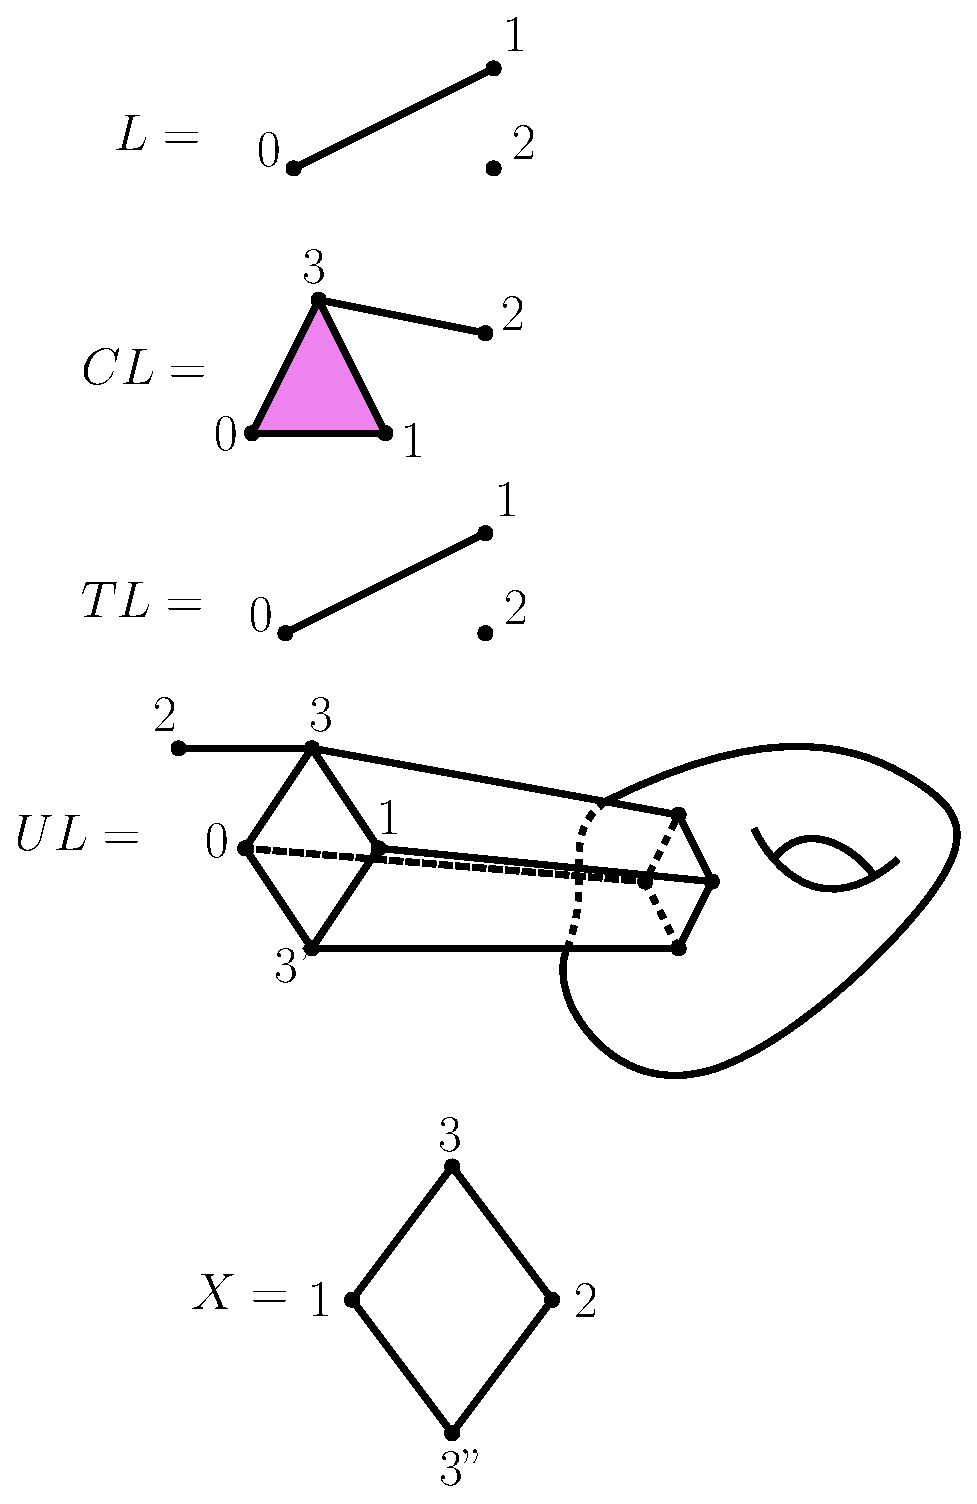
\includegraphics[scale=0.7]{pict5}
\caption{}\label{pict_5}
\end{center}
\end{figure}
 

Пространство $TK$ будет представлять собою $[0, 1]\cup [3'', 1]\cup [3'', 2]$ и будет отображаться в $K$, отправляя точку $3''$ в барицентр отрезка $[1, 2]$. В качестве пространства $UK$ будет выступать объединение отрезка $[0, 1]$ и пространства с двумя склеенными копиями $A$, причём вторая копия $A$ будет подклеиваться к <<рогу>> $[3,2]\cup [3, 1]$. 

{\bf Шаг 3.} Приклеим третье ребро $[0, 2]$. В результате, к $UL$ подклеится ещё одна копия пространства типа $A$ с прошлого шага, но уже к рогу $[3, 2]\cup [3, 0]$, также к $UL$ подклеится отрезок $[1, 2]$. Пространство Кана-Тёрстона будет $[0, 1]\cup [1, 2]\cup [3''', 2]\cup [3''', 0]$ --- окружность.



{\bf Шаг 4.} Подклейка двумерной клетки к границе треугольника. Комплекс $T\Delta^2$ будет представлять собой три образования типа $A$, склеенных вдоль трёх рогов с общей вершиной $[3]$ и остальными вершинами $[0], [1], [2]$. См. схему расположения <<рогов>> на рис. \ref{pict_7}.

\begin{figure}
\begin{center}
\includegraphics[scale=0.7]{pict7}
\caption{}\label{pict_7}
\end{center}
\end{figure}

Как устроено отображение $t: TK\to K$? Конус над границей треугольника $[0, 1, 2]$ с вершиной $[3]$ переходит в треугольник $[0, 1, 2]$ так, что вершина $[3]$ отображается в барицентр треугольника $[0, 1, 2]$, а остальные вершины конуса переходят тождественно в вершины этого треугольника. На другие точки этого конуса отображение $t$ продолжается по линейности. На каждом из трёх подклееных цилиндров отображение $t$ уже задано.    
 
Полученное пространство $T\Delta^2$ имеет в качестве фундаментальной группы свободное произведение трёх групп Хигмана $\Hig_4$. То есть для стягиваемых пространств конструкция Маундера даёт нестягиваемые ацикличные пространства. Это наглядно иллюстрирует тот факт, что функтор Кана-Тёрстона не является гомотопическим.

Видно также, что уже для такого пространства, как двумерный симплекс, возникают трудности с явным построением его пространства Кана-Тёрстона уточнённым методом Маундера.








\subsubsection{Группа $\mathfrak{U}$ и функтор Маундера}\label{modification}

Как было видно из \S\ref{construction_for_triangle}, с уточнённой конструкцией Маундера функтора $T$ достаточно неудобно работать.

Из следствия \ref{AcyclUniv} теоремы \ref{BousfUniv} получается, что в основной конструкции Маундера в качестве гомологического конуса будет годиться универсальная конечно определённая ацикличная группа $\mathfrak{U}$ (см. \S\ref{SectionUnivAcyclGroup}). В обозначениях этой конструкции $\pi_1(T\partial\sigma) = \pi$ вкладывается в $C\pi := \mathfrak{U}$ и затем к $T\partial\sigma$ приклеивается цилиндр отображения $T(\partial\sigma)\to K(\mathfrak{U}, 1)$. Однако если исходно мы имели конечный симплициальный комплекс $X$, то в результате получится бесконечномерный симплициальный комплекс $TX$ с конечным числом клеток каждой размерности, поскольку группа $\mathfrak{U}$ имеет кручение (см. \S\ref{SectionUnivAcyclGroup}). Тем не менее, группа $\mathfrak{U}$ решает проблему вложения группы в её гомологический конус в общей конструкции Маундера.





\subsubsection{Функтор Маундера для двумерных комплексов}\label{two_complex}

В дальнейшем мы будем применять функтор $T$ к полиэдральным разбиениям двумерных комплексов, поэтому в этом контексте мы будем использовать следующую конструкцию $T$. Рассмотрим общую конструкцию Маундера и в момент подклейки двумерного симплекса будем использовать в качестве гомологического конуса группы $\mathbb{Z}$ группу Хигмана $\Hig_4$.













\subsubsection{Проблема однозначности конструкции Маундера}

Рассмотренные функторы $T$ типа Кана-Тёрстона существенным образом зависят от симплициального разбиения исходного пространства $X$, а также от выбора групповых конусов. Пример уточнённой конструкции Маундера $T\Delta^2$ из \S\ref{construction_for_triangle} показывает, что $T$, вообще говоря, не является гомотопическим функтором. Однако это означает, что если зафиксировать выбор вложения в групповой конус (например, как это сделано в \S\ref{modification} для произвольных комплексов или в \S\ref{two_complex} для двумерных комплексов), то фундаментальная группа пространства $TX$ будет некоторым образом характеризовать комбинаторику исходного симплициального комплекса $X$.    













\section{Группы, свободно действующие на ацикличных пространствах}


Рассмотренные выше функторы Дрора $A$ и Кана-Тёрстона $T$ дают надежду на обобщение понятия универсального расслоения. А именно, для данной группы $G$ зададимся поиском ацикличного, но не стягиваемого пространства $\mathcal{E}G$, на котором дискретная группа $G$ действует свободно.

Может показаться, что из естественности функтора Дрора может следовать то, что он переводит накрытия симплициальных множеств в накрытия или что композиция $A\widetilde{X}\to \widetilde{X}\to X$ является накрытием. Однако оба этих предположения неверны, поскольку имеет место следующее

\begin{statement}\label{BG}
Если $\mathcal{E}G\to \mathcal{B}G$ --- $G$-накрытие с гомологически тривиальным $\mathcal{E}G$, то $\mathcal{B}G$ имеет такие же гомологии с коэффициентами в тривиальном $G$-модуле $\mathbb{Z}$, как и $BG$ --- классифицирующее пространство группы $G$.
\end{statement}

\begin{proof}
Рассмотрим спектральную последовательность Картана-Лере $$H_p(G; H_q(\mathcal{E}G))\Rightarrow H_\ast(\mathcal{B}G).$$ Она вырождается во втором члене, поэтому $$H_n(\mathcal{B}G)\cong H_n(G; H_0(\mathcal{E}G)) = H_n(G; \mathbb{Z}) = H_n(G).$$ Последнее равенство верно в силу тривиальности $G$-модуля $\mathbb{Z}$.
\end{proof}

Похожий естественный вопрос возникает и для функторов Кана-Тёрстона: существует ли такая конструкция функтора Кана-Тёрстона $T$, что если $\widetilde{X}\to X$ является $G$-накрытием, то $T\widetilde{X}\to TX$ тоже является $G$-накрытием. Оказывается, функтор Маундера, рассмотренный в \S\ref{Maunder}, является искомым, то есть справедлива

\begin{theorem}\label{RespectCovering}
Существует функтор типа Кана-Тёрстона, переводящий $G$-накрытия в $G$-накрытия.
\end{theorem}

\begin{proof}
Пусть отображение симплициальных комплексов $Y\to X$ является $G$-накрытием, т. е. на пространстве $Y$ задано свободное симплициальное действие дискретной группы $G$, такое, что в факторе $Y/G$ получается пространство $X$. Покажем, что по действию $G\curvearrowright Y$ можно построить действие $G$ на конструкции Маундера пространства Кана-Тёрстона $TY$. Поскольку $\mathrm{sk}^1 TY = Y$, то на одномерном остове действие $G$ уже задано. Предположим теперь, что мы подклеиваем к комплексу $L\subset Y$ некоторую клетку $\sigma$ и мы смогли уже задать действие $G$ на $TL$. Приклейке клетки $\sigma$ соответсвует приклейка цилиндра $\mathrm{Cyl} = \mathrm{Cyl}\, \left (T(\partial \sigma)\to K(C\pi_1(T\partial\sigma), 1)\right )$ к $TL$. Пусть элемент $g$ переводит $T\partial\sigma$ в $T\partial\sigma'$. Тогда будем считать, что $g$ переводит подклеивающийся цилиндр $\mathrm{Cyl}$ в его копию $\mathrm{Cyl}'$, которая, в свою очередь, будет подклеиваться к $T\sigma'$. Таким образом можно продолжить действие с орбиты $T\sigma$ на подклеенные цилиндры и значит, в конечном счёте на всё пространство $TY$.   
\end{proof}

\begin{corollary}
Для любой дискретной группы $G$ существует ацикличное нестягиваемое пространство $\mathcal{E}G$ со свободным действием группы $G$. Факторпространством по этому действию будет пространство $\mathcal{B}G$, гомологически эквивалентное классифицирующему пространству $BG$ группы $G$.
\end{corollary}

\begin{proof}
Достаточно применить теорему \ref{RespectCovering} к универсальному накрытию $\mathcal{E}G\to\mathcal{B}G$. Гомологическая эквивалентность $\mathcal{B}G$ и $BG$ следует из утверждения \ref{BG}. 
\end{proof}


Рассмотрим категорию $\mathbf{Acyc}$, объектами которой являются ацикличные $G$-пространства, а морфизмами --- эквивариантные $G$-отображения.

Имеется следующий 

\begin{question}
Существует ли конструкция функтора $T$, для которой объект $\mathcal{B}G$ был бы терминальным в категории $\mathbf{Acyc}$?
\end{question}
















\section{Полиэдры и конечно определённые группы}

Предположим, что топологическое пространство $X$ представлено в виде разбиения $P$ на выпуклые многогранники, возможно, разных размерностей. Тогда функтор Маундера по фиксированному выбору ацикличных групп в его конструкции ставит в соответствие разбиению $P$ асферичное пространство $TP$ и, в частности, фундаментальную группу $\pi_1 TP$. Итак, для фиксированной конструкции функтора $T$, мы имеем соответствие $$P\mapsto \pi_1TP.$$ 















\subsection{Конструкция $\boldsymbol{TP}$ для 3-полиэдров $\boldsymbol{P}$}

Для выпуклых трёхмерных многогранников $P$ конструкцию можно уточнить:

\begin{itemize}

\item Для этого выберем в 1-остове $P$ максимальное дерево (на рисунках будем обозначать его фиолетовым цветом). 

\item Оставшиеся рёбра будут тогда образующими фундаментальной группы 1-остова многогранника (на рисунках им будут отвечать красные рёбра).

\end{itemize}

Для дальнейшего нам понадобится

\begin{defi}
{\it Пунктированная конечно определённая группа} --- группа с выделенной образующей.
\end{defi}

\begin{itemize}


\item Рассмотрим $f$ копий пунктированных групп Хигмана $$\Hig^i_4 = \langle a_i, b_i, c_i, d_i\ | \ ... \rangle,\ i=1,..., f$$ где $f$ --- число граней многогранника $P$ и в каждой группе $\Hig^i_4$ выбрана образующая $a_i$.

\item Приклеим цилиндр отображения $\partial F_i → K (\Hig^i_4, 1)$ к границе грани $F_i$ в 1-остове $P$ для каждой группы Хигмана $\Hig^i_4$ ($i = 1, ..., f$). Здесь $\partial F_i$ представляет собой окружность, и она отождествляется с окружностью, соответствующей образующей $a_i$ в группе Хигмана $\Hig^i_4$. Подразбивая 1-остов в комплексе $K(\Hig_4, 1)$, если нужно, мы сможем реализовать нужные отождествления.

\end{itemize}











\begin{example}

Найдём фундаментальную группу пространства $TL$, где $L$ --- минимальное симплициальное разбиение $\mathbb{S}^2$, отвечающее тетраэдру, см. рис. \ref{pict_tetrahedron}.      
 
 \begin{figure}
 \begin{center}
\includegraphics[scale=0.8]{tetrahedron}
\caption{}\label{pict_tetrahedron}
\end{center}
\end{figure}

Рассмотрим 1-остов $\mathrm{sk}^1\, L$ тетраэдра $SX_1X_2X_3$. Будем считать точку $S$ отмеченной в этом комплексе. Обозначим через $x_1, x_2$ и $x_3$ классы гомотопий петель $S\to X_2\to X_3\to S$, $S\to X_3\to X_1\to S$ и $S\to X_1\to X_2\to S$ соответственно. Стягивая одномерный подкомплекс на вершинах $S, X_1, X_2$ и $X_3$, мы получаем, что фундаментальная группа 1-остова тетраэдра имеет следующее копредставление $$\pi_1(\mathrm{sk}^1\, L, S) = \langle x_1, x_2, x_3 \rangle,$$ т. е. является свободной группой $F_3$ ранга 3 на элементах $x_1, x_2$ и $x_3$.

Занумеруем грани тетраэдра так, что грань $X_1X_2X_3$ соответствует 4-й грани, а любая другая грань имеет номер $j$, если она примыкает к отмеченному буквой $x_j$ ребру.  

При подклеивании цилиндра $f_{4}$ к четвёртой грани слово $x_1 x_2 x_3$ в группе $\pi_1(\mathrm{sk}^1\, L, S)$ можно отождествить, например, с образующей $a_4$ группы Хигмана $$\Hig_4 = \langle a_4,b_4,c_4,d_4\ |\ a_4^{-1}b_4a_4 = b_4^2, \ b_4^{-1}c_4b_4 = c_4^2, \ c_4^{-1}d_4c_4 = d_4^2, \ d_4^{-1}a_4d_4 = a_4^2 \rangle.$$

После подклеивания цилиндра к грани $X_3X_1X_2$ фундаментальная группа будет иметь вид $$F_3\star_{\mathbb{Z}}\Hig_4 =$$ $$ \langle x_1, x_2, x_3, a_4, b_4, c_4, d_4\ | $$ $$\ a_4 = x_1x_2x_3, (a_4)^{-1}b_4(a_4) = b_4^2,\ b_4^{-1}c_4b_4 = c_4^2,\ c_4^{-1} d_4c_4 = d_4^2, \ d_4^{-1} a_4d_4 = a_4^2 \rangle.$$

Осталось ещё приклеить 3 цилиндра к оставшимся граням. Для первой грани мы будем иметь отождествление по слову $x_1$. Значит, при подклеивании нового цилиндра возникнет свободное произведение с изоморфной копией $\Hig_4$ с отождествлением элемента $x_1$ вдоль элемента $a_1$. К имеющемуся копредставлению группы $F_3\star_\mathbb{Z}\Hig_4$ добавятся образующие $a_1, b_1, c_1, d_1$ и соотношения из группы Хигмана на этих образующих, плюс соотношение склейки $x_1 = a_1$. 

Рассуждая аналогичным образом для оставшихся граней, получаем, что фундаментальная группа комплекса $TL$ будет иметь копредставление, в котором образующими будут $a_i, b_i, c_i$ и $d_i$ для $i = 1, 2, 3, 4$ и также $x_j$ для $j = 1, 2, 3$. Первая группа образующих для каждого фиксированного $i$ соответствует образующим группы Хигмана для $i$-й грани тетраэдра. Множество соотношений для данной группы будет являться объединением множеств соотношений для четырёх групп Хигмана $\Hig_4$ и отождествлений вдоль произведений отмеченных рёбер каждой грани. Более конкретно, нужно объединить множество $$\bigcup\limits_{i=1}^4\left\{ [b_i, a_i] = b_i,\ [c_i, b_i] = c_i,\ [d_i, c_i] = d_i,\ [a_i, d_i] = a_i\right\},$$ где $[x, y] = x^{-1}y^{-1}xy$, а также множество $$\left\{ x_1x_2x_3 = a_1,\ x_k = a_k,\ k = 1, 2, 3 \right\}.$$

Итого, мы получаем группу с $4\cdot 4 + 3 = 19$ образующими и $4\cdot 4 + 1 + 3 = 20$ соотношениями.


\end{example}







Обозначим эйлерову характеристику трёхмерного полиэдра $P$ через $\chi(P)$. Тогда для этого полиэдра $v - e + f = \chi(P)$, где $v, e$ и $f$ обозначают числа вершин, рёбер и граней $P$. Для 1-остова $P$ получаем, что $\chi(\mathrm{sk}^1\, P) = v - e = \chi(P) - f$. После стягивания в точку остовного дерева у 1-остова $P$ мы будем иметь одну вершину и $e'$ рёбер, но ту же эйлерову характеристику $\chi(\mathrm{sk}^1\, P)$. Откуда получаем, что $e' = f - \chi(P) + 1$ --- число рёбер вне остовного дерева. Значит, копредставление фундаментальной группы пространства Кана-Тёрстона для данного комплекса будет иметь $e' + 4f = 5f - \chi(P) + 1$ порождающих и $f + 4f = 5f$ соотношений. 

В частности, для многогранников $P\cong \mathbb{S}^2$ мы получим конечно определённую группу $\pi_1TP$, имеющую $5f - 1$ образующих и $5f$ соотношений.














\begin{example}    

Рассмотрим замощение проективной плоскости шестью пятиугольниками, см. рис. \ref{pict_dodecahedron}. 

\begin{figure}
\begin{center}
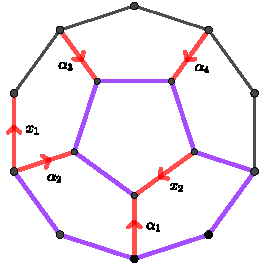
\includegraphics[scale=1.9]{Dodecahedron.pdf}
\caption{}\label{pict_dodecahedron}
\end{center}
\end{figure}


На рисунке предполагается отождествление симметричных относительно центра сторон 10-угольника. Фиолетовым цветом выделено максимальное дерево 1-остова комплекса, которое предполагается стягивать. Красные отрезки являются образующими фундаментальной группы 1-остова. Фундаментальная группа соответствующего пространства Кана-Тёрстона имеет копредставление с образующими $x_1, x_2, \alpha_i$, $i=1,..., 4$, $a_j, b_j, c_j, d_j$, $j=1, ..., 6$. Нумерация групп Хигмана соответствует следующей нумерации граней. Пусть центральная грань имеет номер 6, а остальные грани занумерованы против часовой стрелки, начиная с грани с рёбрами $x$ и $\alpha_1$. Соотношения получаются объединением соотношений для шести групп Хигмана, а также соотношений, соответствующих склейке слов в каждой грани с образующими групп Хигмана: 


\begin{itemize}

\item 5-пояс: $\alpha_1\alpha_2^{-1} = a_1$, $x_2\alpha_1^{-1} = a_2$, $\alpha_4 = a_5$, $x_1\alpha_4 = a_3$, $\alpha_3\alpha_4^{-1} = a_4$, $\alpha_2\alpha_3^{-1}x_1^{-1} = a_5$

\item Центральная грань: $x^{-1} = a_6$

\end{itemize}


Итого, мы имеем $6 + 6\cdot 4 = 30$ образующих и $4\cdot 6 + 6 = 30$ соотношений.    

\end{example}












\begin{example}

Рассмотрим следующее разбиение тора на квадраты, см. рис. \ref{pict_torus}.

\begin{figure}
\begin{center}
\includegraphics[scale=0.8]{Torus}
\caption{}\label{pict_torus}
\end{center}
\end{figure}

Здесь мы будем иметь $9\cdot 4 + 10 = 46$ образующих: $a_i$, $b_i$, $c_i$, $d_i$ ($i = 1, ..., 9$), $x_j$ ($j = 1, ..., 10$) и $9\cdot 4 + 9 = 45$ соотношений: соотношения из групп Хигмана, соотношения склейки при обходе квадратов разбиения.

\end{example}



















\subsection{Многогранники с гамильтоновыми путями}  





Предположим, что 1-остов трёхмерного многогранника $P$ имеет гамильтонов путь $\gamma$. Опишем канонический способ задания группы $\pi_1TP$ образующими и соотношениями:

\begin{enumerate}[\bf 1.]

\item Зафиксируем ориентированный гамильтонов путь $\gamma$ в 1-остове $P$ с нумерацией вершин. Оставшиеся рёбра будем называть красными.

\item Упорядочим лексикографически красные рёбра.

\item Зафиксируем ориентацию многогранника $P$.

\item Отметим по образующей $a_i$ для каждой из $f$ групп Хигмана $\Hig^i_4$.

\item Красные рёбра пометим символами $x_i$, где $i$ является номером красного ребра в лексикографическом порядке.

\item Зададим нумерацию граней и запишем соотношения приклейки последовательно для каждой грани.      

\end{enumerate} 






\begin{example}

Рассмотрим снова тетраэдр, но теперь вместо произвольного дерева выберем гамильтонов путь (он показан фиолетовыми рёбрами), см. рис. \ref{pict_tetrahedron_hamilt}.

\begin{figure}
\begin{center}
\includegraphics[scale=0.8]{tetrahedron_hamilt}
\caption{}\label{pict_tetrahedron_hamilt}
\end{center}
\end{figure}

Запишем соотношения приклейки: $\{ x_1^{-1} = a_1,\; x_2^{-1}x_1 = a_2, \; x_3^{-1}x_2 = a_3, x_3 = a_4 \}$




\end{example}















\section{Приложения к математической теории фуллеренов}

Как было сказано во введении, в химии, физике и нанотехнологиях важной является задача классификации изомеров фуллеренов. В данном разделе описывается алгоритм, который строит по любому фуллерену $P$ конечно определённую группу $G_P$.    

\begin{defi}
{\it Математическим фуллереном} называется выпуклый простой трёхмерный многогранник, все двумерные грани которого являются пяти- и шестиугольниками. 
\end{defi}

Далее, для краткости будем называть фуллеренами математические фуллерены.

Известно \cite{Fullerenes}, что каждый фуллерен имеет ровно 12 пятиугольных граней и $p_6$ шестиугольных, где $p_6$ может принимать любое значение, кроме 1. 

Все количественные комбинаторные данные фуллерена однозначно выражаются через его число шестиугольных граней $p_6$ следующимм образом \cite{Fullerenes}: $$f_0 = 20 + 2p_6,\ f_1 = 30 + 3p_6, \ f_2 = 12 + p_6.$$

Оказывается, 1-остов любого фуллерена является гамильтоновым графом, т. е. он содержит гамильтонов цикл.

\begin{theorem}[F. Kardo\v{s}, 2017, \cite{Kardos}]

Пусть $G$ является $3$-связным планарным кубическим $($все вершины имеют степень $3)$ графом, каждая грань которого является $n$-угольником, где $n\leqslant 6$. Тогда $G$ является гамильтоновым.

\end{theorem}
 

\begin{corollary}

$1$-остов любого фуллерена содержит гамильтонов цикл.

\end{corollary}


Суммируя всё выше сказанное, получаем следующий результат:

\begin{theorem}

Каждому фуллерену $P$ с выбранной ориентацией, по группе Хигмана $\Hig_4 = \langle a, b, c, d\ | \  ... \rangle$ с отмеченной образующей $a$ и по ориентированному гамильтонову пути $\gamma$ можно канонически сопоставить конечно определённую группу $G_P$. 

\end{theorem}





Каждый фуллерен с $p_6$ шестиугольными гранями обозначается символом $P_{p_6, k}$, где $k$ является номером изомера. Оказывается, число изомеров фуллеренов $P_{p_6, k}$ довольно быстро растёт:

\begin{theorem}[W. Thurston, 1998, \cite{Thurston}]
Количество комбинаторно неэквивалентных фуллеренов с $p_6$ шестиугольными гранями имеет рост порядка $p_6^9$.
\end{theorem}
 








\begin{figure}
\begin{center}
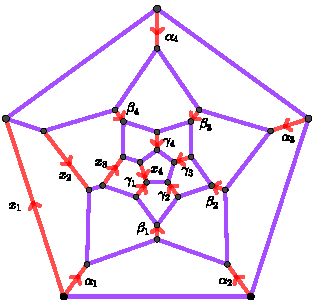
\includegraphics[scale=1.9]{Fullerene}
\caption{}\label{pict_fullerene}
\end{center} 
\end{figure}





\begin{example}

Рассмотрим фуллерен $P_{5, 1}$, см. рис. \ref{pict_fullerene}. Фундаментальная группа пространства Кана-Тёрстона будет иметь своими образующими $a_s, b_s, c_s, d_s$ ($s = 1, ..., 17$), $x_i$ ($i = 1, ..., 4$), $\alpha_j$ ($j = 1, ..., 4$), $\beta_k$ ($k = 1, ..., 4$), $\gamma_\ell$ ($\ell = 1, ..., 4$). К соотношениям в группах Хигмана мы должны добавить ещё соотношения склейки для каждой грани:


\begin{itemize}



 \item Первый 5-пояс: $x_1^{-1}\alpha_1x_2^{-1} = a_1$, $\alpha_{i + 1}\alpha_{i}^{-1} = a_{i + 1}$ ($i = 1, 2, 3$), $\alpha_4^{-1} = a_5$
 
 \item Второй 5-пояс: $x_2x_3\beta_4^{-1} = a_6,$ $\beta_{j + 1}\beta_{j}^{-1} = a_{j + 6}$ ($j = 1, 2, 3$), $\beta_1 = a_{10}$
 
 \item Третий 5-пояс: $\gamma_1x_4^{-1}x_3^{-1} = a_{11}$, $\gamma_{k + 1}\gamma_k^{-1} = a_{k + 11}$ ($k = 1, 2, 3$), $\gamma_4^{-1} = a_{15}$
 
 \item Центральная грань: $x_4 = a_{16}$
 \item Внешняя грань: $x_1 = a_{17}$
 \end{itemize}



Итого, мы имеем $16 + 4\cdot 17 = 84$ образующих и $4\cdot 17 + 17 = 85$ соотношений.

\end{example}














\begin{example}

Рассмотрим два изомера $P_{4, 1}$ и $P_{4, 2}$, см. рис. \ref{pict_P_4}. Выпишем для соответствующих групп $\pi_1TP_{4, 1}$ и $\pi_1TP_{4, 2}$ соотношения приклейки цилиндров к граням.


\begin{figure}
\begin{center}
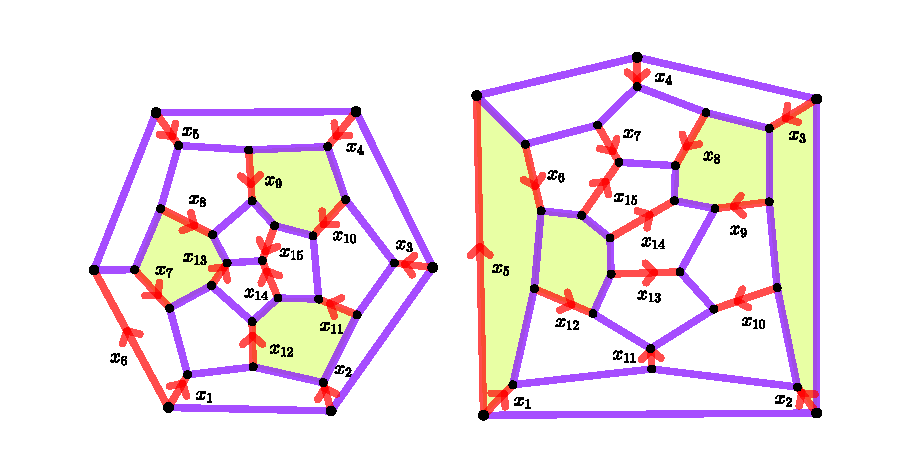
\includegraphics[scale=1.2]{P_4}
\caption{}\label{pict_P_4}
\end{center} 
\end{figure}



\newpage


\begin{center}

\bf Шестиугольные грани

\end{center}

\hrule





\begin{multicols}{2}




\begin{itemize}



\item $x_7x_{13}x_8 = a_1$

\item $x_9x_{10}^{-1} = a_2$

\item $x_{11}x_{12}^{-1} = a_3$

\item $x_6 = a_4$

\end{itemize}

\columnbreak

\begin{itemize}

\item $x_1x_6^{-1}x_5^{-1} = a_1$

\item $x_3x_2^{-1} = a_2$

\item $x_8x_9^{-1} = a_3$

\item $x_{12} = a_4$ 

\end{itemize}


\end{multicols}



\newpage





\begin{center}

\bf Пятиугольные грани

\end{center}

\hrule


\begin{multicols}{2}

\begin{itemize}

\item $x_1x_7^{-1}x_6^{-1} = a_{4}$




\item $x_2x_1^{-1} = a_6$

\item $x_3x_2^{-1} = a_7$

\item $x_4x_3^{-1} = a_8$

\item $x_5x_4^{-1} = a_9$

\item $x_8x_9^{-1} = a_{10}$

\item $x_{10}x_{11}^{-1} = a_{11}$

\item $x_{14}x_{13}^{-1} = a_{12}$

\item $x_{15}x_{14}^{-1} = a_{13}$




\item $x_5^{-1} = a_{14}$

\item $x_{12} = a_{15}$

\item $x_{15}^{-1} = a_{16}$



\end{itemize}

\columnbreak

\begin{itemize}

\item $x_6x_{15}x_7^{-1} = a_5$



\item $x_2x_1^{-1} = a_6$

\item $x_4x_3^{-1} = a_7$

\item $x_7x_8^{-1} = a_8$

\item $x_9x_{10}^{-1} = a_{9}$

\item $x_{11}x_{10}^{-1} = a_{10}$

\item $x_{12}x_{11}^{-1} = a_{11}$

\item $x_{13}x_{14}^{-1} = a_{12}$

\item $x_{14}x_{15}^{-1} = a_{13}$




\item $x_4^{-1} = a_{14}$

\item $x_{13}^{-1} = a_{15}$

\item $x_5^{-1} = a_{16}$


\end{itemize}



\end{multicols}




\begin{question}\label{QUESTION}
Изоморфны ли группы $\pi_1TP_{4, 1}$ и $\pi_1TP_{4, 2}$?
\end{question}

\begin{hypothesis}
Фуллерены $P_1$ и $P_2$ комбинаторно эквивалентны тогда и только тогда, когда имеется изоморфизм групп $\pi_1TP_1\cong \pi_1 TP_2$. 
\end{hypothesis}

Подтверждение данной гипотезы будет означать, что изомеры фуллеренов $\{P\}$ могут быть классифицированы соответствующими конечно определёнными группами $\{\pi_1TP\}$ по аналогии с результатом из торической топологии о кольцах когомологий момент-угол многообразий, соответствующих погореловским многогранникам (см. \S\ref{Introduction}). Однако пока автору не удалось найти ответ даже на вопрос \ref{QUESTION}.   



\end{example}












\section{Выводы и заключение}

Таким образом, в настоящей работе получены результаты об ацикличных группах и пространствах, упомянутые в \S\ref{Introduction}. Для каждого полиэдрального разбиения $P$ топологического пространства $X$ описана конструкция конечно определённой группы $G_P$. В случае фуллеренов приведён канонический вариант этой конструкции, который использует при построении гамильтонов путь, ориентацию фуллерена и выбор пунктированной ацикличной группы.

В процессе работы были сформулированы вопросы и гипотезы. На часть из этих вопросов были даны исчерпывающие ответы, а с остальными автор связывает свою дальнейшую научную работу.   
























































\newpage


\pagestyle{fancy}
\fancyhf{}
\rhead{\thepage}
\lhead{\S\thesection. \leftmark}





\phantomsection

 \addcontentsline{toc}{section}{Список литературы}

\bibliographystyle{plain}
\bibliography{data}




































\end{document}